%%%%%%%%%%%%%%%%%%%%%%%%%%%%%%%%%%%%%%%%%%%%%%%%%%%
%%%%%%%% ICML 2014 LATEX SUBMISSION FILE %%%%%%%%%%
%%%%%%%%%%%%%%%%%%%%%%%%%%%%%%%%%%%%%%%%%%%%%%%%%%%

\documentclass{article}

% do we need this package with icml
%\usepackage{subfigure} 

% Include packages here
% NOT FOR ICML!
%\IEEEoverridecommandlockouts             
%\overrideIEEEmargins

\usepackage{amsthm}
\usepackage{graphicx}
%\usepackage{cite}
\usepackage{url}
\usepackage{epstopdf}
\usepackage{graphics} % for pdf, bitmapped graphics files
\usepackage{epsfig} % for postscript graphics files
\usepackage{times} % assumes new font selection scheme installed

%Thorem environment http://en.wikibooks.org/wiki/LaTeX/Theorems
\newtheorem{prop}{Proposition}[section]
\newtheorem{theorem}{Theorem}[section]
\newtheorem{prop2}{Proposition}
\newtheorem{lem}{Lemma}
% Math related
\usepackage{amssymb}  % assumes amsmath package installed
\usepackage{amsmath} % assumes amsmath package installed
%\usepackage{mathptmx} % assumes new font selection scheme installed

\usepackage[dvipsnames]{xcolor}
\usepackage{transparent}

%matlabpsfrag
\usepackage{pstool}

% For algorithms
\usepackage{algorithm}
\usepackage{algorithmic}

% strike out
\usepackage{soul}


%SVG-Latex Stuff
%%%%%%%%%%%%%%%%%%%%%%%%%%%%%%%%%%%%%%%%%%%%%%%%%%
%%%% Path for your figures
%%%%%%%%%%%%%%%%%%%%%%%%%%%%%%%%%%%%%%%%%%%%%%%%%%
%% Set the paths where all figures are taken from:
\graphicspath{{data/}}
\newcommand{\executeiffilenewer}[3]{%
 \ifnum\pdfstrcmp{\pdffilemoddate{#1}}%
 {\pdffilemoddate{#2}}>0%
 {\immediate\write18{#3}}\fi%
}

\newcommand{\includesvg}[1]{%
% \executeiffilenewer{#1.svg}{#1.pdf}%
% {inkscape -z -D --file=#1.svg %
% --export-pdf=#1.pdf --export-latex}%
 \input{data/#1.pdf_tex}%
}

\newcommand{\note}[1]{{\color{cyan}[Note: #1]}}
\newcommand{\todo}[1]{{\color{ForestGreen}[TODO: #1]}}


% http://tex.stackexchange.com/questions/16429/equation-spanning-two-columns-in-ieeetran
%\usepackage{stfloats}

% dash line
%\usepackage{arydshln}
% cleverref
%\usepackage{cleveref}

% fig2texPS 
\usepackage{pgfplots}
\pgfplotsset{compat=newest} 
\pgfplotsset{plot coordinates/math parser=false}

%%%%%%%%%%%%%%%%%%%%%%%%%%%%%%%%%%%%%%%%%%%%%%%%%%
%%%% Define your own commands here
%%%%%%%%%%%%%%%%%%%%%%%%%%%%%%%%%%%%%%%%%%%%%%%%%%
\newcommand{\Bruch}[2]{{}^{#1}\!\!/\!_{#2}}
\renewcommand{\labelenumi}{\roman{enumi}.)}

%% custom macros
\newcommand{\state}{x} % used to denote the system states
\newcommand{\traj}{s} % used to denote the point on the trj
\newcommand{\Traj}{\Sigma}
\newcommand{\sysInput}{u} % used to denote the system inputs
\newcommand{\context}{c} % used to denote contexts
\newcommand{\cost}{q} % used to denote stage costs
\newcommand{\ctxaction}{z} %used to denote contexts and actions combined
\newcommand{\observations}{\mathbf{y}} % used for the observed output
\newcommand{\dynamics}{f}
\newcommand{\dynamicsNominal}{f_{\mathrm{nom}}}
\newcommand{\policy}{\mathbf{\pi}}
\newcommand{\ValueFunction}{J}
\newcommand{\episode}{\ell} % used for episode number
\newcommand{\numepisode}{L} % total number of episodes
\newcommand{\threshold}{\epsilon_s}
\newcommand{\alg}{\emph{TGP}}
\newcommand{\dataset}{Z}

\newcommand{\aatop}[2]{\genfrac{}{}{0pt}{}{#1}{#2}}
\renewcommand{\theequation}{\arabic{equation}}
%\numberwithin{equation}{subsection}

%\newenvironment{proof}[1][Proof]{\begin{trivlist}
%\item[\hskip \labelsep {\bfseries #1}]}{\end{trivlist}}
\newenvironment{definition}[1][Definition]{\begin{trivlist}
\item[\hskip \labelsep {\bfseries #1}]}{\end{trivlist}}
\newenvironment{example}[1][Example]{\begin{trivlist}
\item[\hskip \labelsep {\bfseries #1}]}{\end{trivlist}}
\newenvironment{remark}[1][Remark]{\begin{trivlist}
\item[\hskip \labelsep {\bfseries #1}]}{\end{trivlist}}

%\newcommand{\qed}{\nobreak \ifvmode \relax \else
%      \ifdim\lastskip<1.5em \hskip-\lastskip
%      \hskip1.5em plus0em minus0.5em \fi \nobreak
%      \vrule height0.75em width0.5em depth0.25em\fi}
      
      
\DeclareMathOperator*{\plim}{plim}
% \def\MR#1{\href{http://www.ams.org/mathscinet-getitem?mr=#1}{MR#1}}


% For citations
\usepackage{natbib}

% As of 2011, we use the hyperref package to produce hyperlinks in the
% resulting PDF.  If this breaks your system, please commend out the
% following usepackage line and replace \usepackage{icml2014} with
% \usepackage[nohyperref]{icml2014} above.\part{title}
\usepackage{hyperref}

% Packages hyperref and algorithmic misbehave sometimes.  We can fix
% this with the following command.
\newcommand{\theHalgorithm}{\arabic{algorithm}}

% Employ the following version of the ``usepackage'' statement for
% submitting the draft version of the paper for review.  This will set
% the note in the first column to ``Under review.  Do not distribute.''
\usepackage{icml2014} 
% Employ this version of the ``usepackage'' statement after the paper has
% been accepted, when creating the final version.  This will set the
% note in the first column to ``Proceedings of the...''
%\usepackage[accepted]{icml2014}

% The \icmltitle you define below is probably too long as a header.
% Therefore, a short form for the running title is supplied here:
\icmltitlerunning{Trajectory Tracking with Gaussian Processes}

\begin{document} 

\twocolumn[
\icmltitle{Gaussian Process Optimization based Learning for Trajectory Tracking}

% It is OKAY to include author information, even for blind
% submissions: the style file will automatically remove it for you
% unless you've provided the [accepted] option to the icml2014
% package.
\icmlauthor{Okan Koc}{okankoc@gmail.com}
\icmlauthor{Mohanarajah Gajamohan}{gajan@ethz.ch}
\icmladdress{Institute of Dynamic systems and Control, Department of Mechanical and Process Engineering, ETH  Zurich, 8092 Zurich, Switzerland}
\icmlauthor{Andreas Krasue}{krausea@ethz.ch}
\icmladdress{Department of Computer Science, ETH Zurich, 8092 Zurich, Switzerland}
% You may provide any keywords that you 
% find helpful for describing your paper; these are used to populate 
% the "keywords" metadata in the PDF but will not be shown in the document
\icmlkeywords{Gaussian process, multi-armed bandits, exploration-exploitation dilemma, nonlinear optimization, trajectory tracking, machine learning, ICML}

\vskip 0.3in
]

\begin{abstract} 
Systems that work in a repetitive manner use Iterative Learning Control (ILC) algorithms to iteratively improve the performance over a given repeated task or trajectory. 
%The feed-forward control signal is modified in each iteration to reduce the error or the deviation from the given reference trajectory. 
The limitation with ILC is that it assumes the task or the trajectory to be fixed over iterations. ILC cannot handle the cases when the trajectory is modified or changing over time, and the %iterative learning 
controller must start learning from scratch. In this paper we present a reinforcement learning algorithm that we call $\alg$, prove its convergence for trajectory tracking and show that a significant amount of knowledge can be transferred even between cases where the reference trajectories are not the same. 
%using CGP-UCB, an intuitive upper-confidence style algorithm based on Gaussian Processes (GP), 

\end{abstract} 

\section{Introduction}

Control systems are designed to regulate the behavior of dynamical systems and make them follow a human-assigned task or trajectory. They base their regulation on a physical \emph{nominal} model, often derived from first principles. However, whenever there is an uncertainty in the model, such as repeating disturbances not taken into account in a complex environment, the control system will need to learn from its past behavior and compensate for the inaccuracy of the nominal model. Machine Learning tools can be employed in an \emph{Adaptive Control} fashion to guide this learning process.

For systems that work in a repetitive manner, such as robotic manipulators and chemical plants, Iterative Learning Control (ILC) algorithms are used to improve on the performance. In ILC, the feed-forward control signal is modified in each iteration to reduce the error or the deviation from the given task or reference trajectory. A good analogy is a basketball player shooting a free throw from a fixed position: during each shot the basketball player can observe the trajectory of the ball and alter the shooting motion in the next attempt \cite{Bristow06}. 

The limitation with ILC is that it assumes a fixed task or trajectory. While this is a reasonable assumption to make in some repeated tasks, ILC is not \emph{learning} in the proper sense: it fails to generalize over different tasks and cannot handle the cases when the trajectories are modified. In all such cases, the Iterative Learning Controller will need to start from scratch, throwing away useful data. Data from different tasks can be used to generalize, a matter of paramount importance in complex tasks. 

We therefore look at the problem of \emph{generalization} and show that a significant amount of knowledge can be transferred even between cases where the reference trajectories are not the same. A basketball player does not have to learn the free throw motion from scratch each time he finds himself in a slightly different position. We call these cases or reference trajectories \textit{contexts}. Context can change in a given task and it is the responsibility of the autonomous agent or the learning controller to adapt to different contexts. 

The motivation for transfer learning under different contexts comes mainly from the RoboEarth project \cite{Waibel11}, a robot specific knowledge repository where robots share and learn from each others' experience.  The ability to transfer knowledge even under different contexts will significantly improve the performance of future robots. %RoboEarth. 
% 
%operating in a certain location 
For example, consider a robot learning to pour tea into a cup and over time perfecting the motion. The learned pouring motion can be uploaded to a central database, marked with the hardware-specifics of the particular robot as well as the size and shape of the teapot as context. Another robot with slightly different hardware, holding a different teapot, can download the stored motion as a prior and adapt it to its particular context, thereby eliminating the need to learn the motion from scratch.

In this paper, we introduce a reinforcement-learning (RL) algorithm called $\alg$ that learns to track trajectories in state space online. $\alg$ stands for \emph{(trajectory) tracking with Gaussian Processes}. Specifically, the proposed algorithm uses Gaussian Process Optimization (GPO) in the bandit setting to track a given trajectory. It implicitly learns the dynamics of the system, and in addition to improving the tracking performance, it facilitates knowledge transfer between different trajectories. 

%In this paper, we look at the trajectory tracking problem where the dynamics of the system is not completely known. Specifically, we propose an algorithm that learns to optimize the stage costs of a discrete time system with repeating disturbances. The proposed algorithm uses Gaussian Process optimization in the bandit setting to track the minimum of the stage costs. By learning to optimize the stage costs we implicitly learn the dynamics of the system, and in addition to improving the tracking performance, our proposed algorithm facilitates knowledge transfer between different trajectories. 

\paragraph*{Related Work.}Gaussian Processes (GP) are increasingly applied in control theory, where they are used to learn the unknown system dynamics.  \citet{Ko07} propose a hybrid-GP approach combined with reinforcement learning to control an autonomous blimp. Their framework requires them to learn the dynamics itself with multiple GP regressions whereas we use GPO to track the global minimum of an unknown, \emph{scalar} cost function, as will be detailed in the next sections. In \cite{Deisenroth11a,Deisenroth11b} the authors first learn the dynamics with GP regression. In the second step policies for a parameterized controller are learnt by propagating through the GP model. This algorithm, called PILCO, involves necessarily long offline calculations and does not have a guarantee for convergence. Unlike PILCO, $\alg$ incorporates feedback and can generalize over different trajectories. Furthermore we prove that $\alg$ converges to the tracked trajectory under mild assumptions.
% as a function of input and context

% update references?
Gaussian process optimization literature proposes several heuristics such as Expected Improvement \cite{Jones01} and Most Probable Improvement \cite{Lizotte07} for trading off exploration and exploitation. The first method with provable sublinear regret was proposed in \cite{Srinivas09} and extended to the contextual setting in \cite{Krause11}. We apply this approach to dynamical systems in this paper.

\paragraph*{Summary.} Our main contributions are as follows:

\begin{itemize}
\item We propose $\alg$, a reinforcement learning algorithm that efficiently learns to track a given trajectory.
\item We prove that $\alg$ under mild assumptions, learns to track the given trajectory arbitrarily well.
\item With $\alg$ we establish a novel connection with \emph{transfer learning} and present a metric to quantify knowledge transfer. % we establish a framework to analyze
\item We show in numerical examples, the proposed approach and evaluate its performance both in trajectory tracking and in transfer learning by comparing with the state of the art control algorithms.
\end{itemize}

% Unnecessary
%The rest of the paper is organized as follows: Sec.~\ref{sec:bground} introduces the methods used throughout the paper and presents related work. The problem statement and the proposed learning algorithm is presented next in Sec.~\ref{sec:ps}, followed by a theoretical analysis in Sec.~\ref{sec:analysis}. We illustrate the efficiency of the approach in Sec.~\ref{sec:numerical_examples} and conclude in Sec.~\ref{sec:conclusion}, pointing also to possible future work.
% why are sections capitalized and abbreviated?
\section{Problem Statement and Background}\label{sec:bground}

Consider the following discrete dynamics:
\begin{equation}
\state_{t+1} = \dynamics(\state_t,\sysInput_t), \quad  t = 0,1, \ldots, N,
\label{eq:readDynamics}
\end{equation}
where $\dynamics$ is Lipschitz continuous in both arguments, $\state_t \in \mathcal{X} \subset \mathbb{R}^n$ is the state of the system at time stage $t$  and $\sysInput_t \in \mathcal{U} \subset \mathbb{R}^m$ is the control input.  

In discrete time trajectory tracking, the control objective is to minimize the cost functional
\begin{equation}
\ValueFunction(\policy) = \sum_{t=1}^{N} d(\state_{t}, \traj_{t}) \label{costDiscrete}
\end{equation}
where the desired states $\traj_{t}$ belong to a given trajectory $\Traj = \{\traj_0, \traj_1, \ldots, \traj_N\}$ at each time stage, $\policy = \{\sysInput_0, \ldots, \sysInput_{N-1}\}$, and $d(\state_{t}, \traj_{t})$ is a suitably chosen semimetric, e.g. squared Euclidean distance. Note that this minimization should be done considering the state and input constraints and should satisfy \eqref{eq:readDynamics}. In general minimizing \eqref{costDiscrete} is impractical and in Model Predictive Control (MPC), a very popular technique in control theory, the objective to minimize is instead $\sum_{t=1}^{M} d(\state_{t}, \traj_{t})$~\footnote{We discard here the penalties on the inputs $\sysInput_t$.} with $M$ typically much less than $N$, i.e. $M \ll N$.

% receding horizon approaches?
However such receding horizon approaches may perform badly or suffer from instability when the dynamics $\dynamics$ is not known very well. More precisely, consider the following dynamics typically derived from first principles:
\begin{equation}
\hat{\state}_{t+1} = \dynamicsNominal(\state_t,\sysInput_t), \quad  t = 0,1, \ldots, N,
\label{nominal_model}
\end{equation}
where $\dynamicsNominal$ is again Lipschitz continuous in both arguments. This \emph{nominal} model may not be quite accurate when there are unmodelled dynamical effects or repeating disturbances not taken into consideration: \eqref{nominal_model} can fail to predict the future states. The foremost aim of this work is to develop a framework that can learn these unmodelled dynamical effects efficiently. To do this we learn to track at each time stage $t$ the (global) minimum of an unknown scalar cost function $\cost_{t} = d(\state_{t},\traj_{t})$. 

The unknown cost function $\cost_{t} = d(\state_{t},\traj_{t})$ at each time stage $t \geq 1$ depends on the previous state $\state_{t-1}$ and the desired state $\traj_{t}$ as the \emph{context}, the previously applied input $\sysInput_{t-1}$ as the \emph{action}. The contexts $\context_t = (\state_{t}, \traj_{t+1})$ for $t \geq 0$ in a more general setting can be imagined as revealed by an adversary from  $\mathcal{C} = \mathcal{X}^{2}$, i.e. environmental variables independent of the input $\sysInput_t$ to be applied. For brevity we sometimes use the notation $\ctxaction = (\sysInput;\context)$ for the variables in the joint input-context space $\mathcal{D} = \mathcal{U} \times \mathcal{C}$.

\paragraph*{Regret.} A natural performance metric for an algorithm tracking the (global) minimum of a function $\cost(\sysInput;\context)$ is the cumulative regret $R_{T} = \Sigma_{t = 1}^{T}r_{t} $ or equivalently the cumulative reward (the negative of cumulative regret). Here $r_{t} = \cost(\sysInput_{t};\context_{t}) - \cost^{*}$ is the instantaneous regret where $\sysInput_t$ is the action taken at time $t$, $\cost^{*} = \min_{\sysInput \in \mathcal{U}}\cost(\sysInput;\context_t)$.

A desired feature of such an algorithm is to have asymptotically \emph{no-regret}: $\lim_{T \to \infty}R_{T}/T = 0$ because then a subsequence of actions taken converge to the optimal action. Furthermore, any bounds on the average regret $R_{T}/T$ after $T$ rounds imply a convergence rate for this subsequence since the minimum $\min_{t \leq T}\cost(\sysInput_t;\context_t)$ is sandwiched between $\cost^{*}$ and the average. 

\paragraph*{Gaussian Processes and RKHS.} In order to guarantee no-regret, it is necessary to impose some sort of smoothness assumptions on the function $\cost(\sysInput;\context)$. We can implicitly enforce smoothness on the function by assuming that $\cost(\sysInput;\context)$ has low \emph{complexity} as measured under an RKHS norm. \emph{Reproducing kernel Hilbert spaces} \cite{Wahba90} are intimately tied to GPs and their covariance functions $k(\ctxaction,\ctxaction')$. A \textit{Gaussian Process} (GP) is a collection of dependent random variables, any finite number of which has a joint Gaussian distribution \cite{Rasmussen06}. 

%We have used Gaussian Processes for cost function prediction and knowledge transfer between different contexts. 
Gaussian processes, completely specified by a mean function $\mu(\ctxaction)$ and a covariance function $k(\ctxaction,\ctxaction')$, can be seen as a prior distribution over the space of functions. For $y_i = \cost(\ctxaction_i) + \epsilon_i$, $\epsilon_i \sim \mathcal{N}(0,\sigma_{n}^{2})$ with noisy observations $\observations_{T} = \{y_1,\ldots,y_T\}$ at sample points $Z_{T} = \{\ctxaction_1,\ldots,\ctxaction_T\}$, the posterior over $\cost(\ctxaction)$ is again a Gaussian Process distribution with mean $\mu_T{(\ctxaction)}$ and covariance $k_T(\ctxaction,\ctxaction')$ given by the following simple analytic equations:
\begin{align}
\mu_T{(\ctxaction_{*})} &= \mu(\ctxaction_{*}) + \mathbf{k}_T(\ctxaction_{*})^{\mathrm{T}}[\mathbf{K}_T + \sigma_{n}^{2}\mathbf{I}]^{-1}(\observations_T - \boldsymbol{\mu}_T) \label{gpUpdate_mu} \\ 
k_T(\ctxaction_{*},\ctxaction'_{*}) &= k(\ctxaction_{*},\ctxaction'_{*}) - \mathbf{k}_T(\ctxaction_{*})^{\mathrm{T}}[\mathbf{K}_T + \sigma_{n}^{2}\mathbf{I}]^{-1} \mathbf{k}_T(\ctxaction'_{*}) \label{gpUpdate_covar} \\
\sigma_T^{2}(\ctxaction_{*}) &= k_T(\ctxaction_{*},\ctxaction_{*}) \label{gpUpdate_sigma}
\end{align}
where $\boldsymbol{\mu}_T = [\mu(\ctxaction_1),\ldots,\mu(\ctxaction_T)]^\mathrm{T}$ is the prior mean at the sample points, $\mathbf{k}_T(\ctxaction_{*}) = [k(\ctxaction_1,\ctxaction_{*}),\ldots,k(\ctxaction_T,\ctxaction_{*})]^\mathrm{T}$ is the vector of covariances between the sample points and the test point $\ctxaction_{*}$ and $\mathbf{K}_T = [k(\ctxaction,\ctxaction')]_{\ctxaction,\ctxaction' \in Z_T} \succeq 0.$

%The mean update equation \eqref{gpUpdate_mu} is a linear predictor because the resulting mean $\mu_N{(x)}$ is a linear combination of noisy observations $\observations_N$. In the covariance update equation \eqref{gpUpdate_sigma} the quantity $\mathbf{k}_N(x)^{\mathrm{T}}[\mathbf{K}_N + \sigma^{2}\mathbf{I}]^{-1} \mathbf{k}_N(x')$ corresponds to the \emph{information gain} from the noisy observations, i.e. reduction in uncertainty from the prior covariance $k(x,x')$.

With these update equations, Gaussian processes can be used in nonparametric regression to predict the mean and variance of unknown test points. Nonparametric regression methods have the advantage of avoiding rigidity
%overfitting issues 
encountered typically in regression with finite basis functions. 
%The prior models specified by the mean and variance functions are chosen among a discrete set of possible model structures  $\mathit{H_i}$ (including composites). Their \textit{hyperparameters} can be optimized using likelihood functions for training data. The likelihood function specifies the probability of the noisy training data $\observations$ given the sample points $X = \{x_1,\ldots,x_N\}$ and the latent function $f$, seen as a realization of a GP with corresponding hyperparameters. 

%Gaussian Processes when used in estimation, have the advantage of capturing the entire distribution over future values of the function instead of merely their expectation \cite{Rasmussen04}, but unlike Kalman filters require $O(N^3)$ complexity due to the prohibitive matrix inversion in (\ref{gpUpdate_mu}) and (\ref{gpUpdate_sigma}). 
%Several reduced-rank approximations are reported in the literature \cite{Rasmussen06} to overcome the problem of growing $N$ especially in big datasets.

The RKHS $\mathcal{H}_{k}(\mathcal{D})$ corresponding to the GP covariance function $k(\ctxaction,\ctxaction')$ is a complete subspace of $L_{2}(\mathcal{D})$ with an inner product $\langle \cdot,\cdot \rangle_{k}$ obeying the reproducing property: $\langle \cost(\cdot), k(\ctxaction,\cdot) \rangle_{k} = \cost(\ctxaction)$ for all $\cost(\sysInput;\context) \in \mathcal{H}_{k}(\mathcal{D})$. The induced RKHS norm $\|\cost(\sysInput;\context)\|_{k} < \infty$ measures the smoothness of $\cost(\sysInput;\context)$. %The functions $\cost(\sysInput;\context)$ drawn from a GP, i.e. $\cost(\ctxaction) \sim GP(0,k(\ctxaction,\ctxaction'))$ are \emph{almost surely} outside this space of smooth functions \cite{Wahba90} but the linear predictor \eqref{gpUpdate_mu}, being their expectation at time $T$, always falls inside $\mathcal{H}_{k}(\mathcal{D})$.

\paragraph*{Bandits.} In the general reinforcement learning problem, contexts depend on the actions taken. In particular, in trajectory tracking, next states are determined by the previously applied input sequence. A simpler setting where the actions do not influence the contexts is known as \emph{multi-armed bandits}, where in order to find the global minimum of an unknown noisy function, it must be \textit{explored} by sampling at promising points $\sysInput$ and must be \textit{exploited} at the current minimum values. Using upper confidence bounds (UCB) is a particularly simple and intuitive heuristic to balance the exploration/exploitation tradeoff and works by keeping track of upper confidence bounds of the sample points \cite{Srinivas09}. 
%When applied to dynamical systems, the sample points are the control signals and the function to be \emph{minimized} is the cost function. 
%Although the cost function with respect to the system output is well defined, the cost corresponding to the control signal is not completely known due to modeling errors and unknown external disturbances. Therefore, multi-armed bandits can be used to track the global minimum of this cost function while providing a framework that can be extended for knowledge transfer.

%In addition to the controller input, \emph{contexts} such as the current internal state of the system, the current environment state, and desired state can be parameterized in the cost function. 
%Learning over the joint space of inputs and contexts enables the knowledge transfer between 
%different learning controllers with 
%different contexts. 
%With the addition of context, bandit problems transform into a reinforcement learning problem \cite{Sutton98}. 

Krause and Ong in \yrcite{Krause11} discuss such a learning algorithm which maintains a GP-estimate of the function to be optimized with \eqref{UCB}:

\begin{equation}
\sysInput_{t} = \operatorname*{arg\,min}_{u \in U} \big(\mu_{t-1}(\sysInput;\context) - \beta_t^{1/2}\sigma_{t-1}(\sysInput;\context) \big)
\label{UCB}
\end{equation}
where $\beta_t$ is the parameter that balances exploration-exploitation at each time stage $t$. They show that the performance of this algorithm can be linked to the \emph{maximal information gain} for the particular cost function to be learned:

\begin{align}
\gamma_{T}  &= \max_{A \subset \mathcal{D}: |A| = T} \mathcal{I}(\observations_{A};\cost) \\
&= \max_{A \subset \mathcal{D}: |A| = T} H(\observations_{A}) - H(\observations_{A}|\cost)
\end{align}

where $\mathcal{I}(\observations_{A};\cost)$ is the \emph{information gain due to sampling} $A$. For a Gaussian, the entropy $H(\mathcal{N}(\boldsymbol{\mu},\mathbf{K})) = \frac{1}{2}\log|2\pi e \mathbf{K}|$ using which we get: $\gamma_T = \frac{1}{2}\log|\mathbf{I} + \sigma_n^{-2}\mathbf{K}_{A}|$.

The cumulative regret of \eqref{UCB} can be bounded if $\cost(\sysInput; \context) \in \mathcal{H}_k(\mathcal{D})$, i.e. $\|\cost(\sysInput; \context)\|_{k}^{2} \leq B$ for some $B < \infty$, where the kernel generating the RKHS is any valid combination of linear or squared exponential~\footnote{Mat\'{e}rn kernels with $\nu > 1$ can also be considered.} covariance function $k(\ctxaction,\ctxaction')$. The valid combinations of kernels are summarized in \cite{Bishop07}. In particular, tensor products and sums of linear and squared exponential kernels are allowed in our case. The bound on the cumulative regret is as follows:
\begin{align}
R_T = \sum_{t=1}^{T}\cost(\sysInput_{t}; \context_{t}) - \cost^{*} \leq \sqrt{\kappa T \beta_{T} \gamma_{T}} \label{cum-regret}
\end{align}
with high probability $p \geq 1- \delta$. Here $\kappa = 8/\log(1 + \sigma_b^{-2})$ with $\sigma_b$ a uniform bound on the noise. Note that unlike in the Bayesian update equations \eqref{gpUpdate_mu} -- \eqref{gpUpdate_sigma}, \cite{Krause11} makes distribution-free assumptions on the noise variables $\varepsilon_t$ if $\cost(\sysInput; \context) \in \mathcal{H}_k(\mathcal{D})$: they can be an arbitrary martingale difference sequence ($\mathbb{E}[\varepsilon_t|\boldmath{\varepsilon_{<t}}] = 0$ for all $t \in \mathbb{N}$) uniformly bounded by $\sigma_b$. 

The exploration-exploitation parameter $\beta_T = 2B + 300\gamma_{T}\log^{3}(T/\delta)$ depends on $\gamma_T$, the free parameter $\delta$ and the bound $B$. The intuition behind these dependencies is that as the cost function $\cost(\sysInput;\context)$ starts to vary more often with respect to the actions $\sysInput$ or the contexts $\context$, the RKHS-bound penalizing this function will increase. $\beta_T$ will increase and \eqref{UCB} will end up exploring $\mathcal{U}$ more frequently to track the global minimum of this cost function. We will be more \emph{sure} of finding the global minimum if we decrease $\delta$: this will likewise correspond to an increasing exploration rate as $\beta_T$ increases.
\section{Algorithm \alg}\label{sec:algorithm}

%When the dynamics is sufficiently well learned, the learned stage cost might be rolled-out as in MPC over a suitable horizon to provide more stable trajectory tracking and approximate the minimization of the cost functional in \eqref{costDiscrete}.
%Tracking the minimum of the would result in solving the following optimization problem at each time stage:
%\begin{align}
%\sysInput_{t} &= \operatorname*{arg\,min}_{\sysInput \in U} \cost_{t+1}(\state_{t}, \sysInput) \\
%\state_{t+1} &=  \mathbf{f}(\state_t,\sysInput_t) \label{eq:realDynamics_discrete}
%\end{align}
%%where $U \subset \mathbb{R}^m$ is the feasible input space at time stage $t$.
%But system dynamics $\mathbf{f}$ in (\ref{eq:realDynamics_discrete}) is not known. 
%Since we have a nominal model, we can learn $\mathbf{f}$ indirectly by just learning the difference in cost predicted by the nominal model and the actual cost:

The scalar cost $\cost(\sysInput;\context)$ is a function of inputs and contexts, and learning to minimize this function from scratch can be very impractical in most cases, due to the high-dimensionality of the state space. If we have a nominal model \eqref{nominal_model} at hand however, we can use the costs predicted by the nominal model. Hence the strategy that we follow in $\alg$ strikes a different balance between exploration and exploitation as opposed to \eqref{UCB}: we \emph{exploit} \eqref{nominal_model} from the very start, using the nominal model predicted cost $\hat{\cost}(\sysInput_t;\context_t) = d(\hat{\state}_{t+1},\traj_{t+1})$, a known function of $\sysInput_t$, as a prior. 
We \emph{explore} only the difference in cost predicted by the nominal model and the actual cost:
\begin{equation}
\delta \cost_{t+1} = d(\state_{t+1},\traj_{t+1}) - d(\hat{\state}_{t+1},\traj_{t+1}) \label{eq:deltaC}
\end{equation}

%\begin{equation}
%\sysInput_{t} = \operatorname*{arg\,max}_{\sysInput \in U}\mu_{t-1}(\sysInput;\context_t) + \beta_{t}^{1/2}\sigma_{t-1}(\sysInput;\context_t) \label{ucb}
%\end{equation}
%where $\mu_{t-1}$ and $\sigma_{t-1}$ are the posterior mean and standard deviation of the GP over the joint input-context space $U \times C$, and $\beta_{t}$ is the confidence parameter scaling exploration vs. exploitation for the particular problem. Thus, when presented with context $\context_t$, this algorithm uses GP-inference in (\ref{gpUpdate_mu}) and (\ref{gpUpdate_sigma}) to predict the mean and variance for each possible action $\sysInput$, conditioned on all the past observations. 

With $\alg$ we adapt the greedy approach of \eqref{UCB} to the reinforcement learning case, and analyze its performance in trajectory tracking. See Figure \ref{fig:drawing2} for an illustration. Pseudocode for $\alg$ is provided in Algorithm~\ref{alg1}. $\alg$ at each time stage $t\geq 0$ uses the GP-update equations \eqref{gpUpdate_mu} -- \eqref{gpUpdate_sigma} over the joint input-context space $\mathcal{D} = \mathcal{U} \times \mathcal{C}$. It is conditioned on the sets $Z_{T-1}$ and $\observations_{T-1}$ acquired through sampling \eqref{UCB} at $t = (0,1,\ldots,T-1)$ with $\hat{q}(\sysInput;\context)$ added as a known mean function $\mu(\ctxaction)$ in \eqref{gpUpdate_mu}. 

\begin{figure}
	\centering
	\def\svgwidth{\columnwidth}
	\includesvg{figure2_pointTracking}
	\caption{Illustrating trajectory tracking: $\state$ pursuing $\traj$. The gray areas depict the \emph{reachable} regions from the states $\state_{t-1}$ and $\state_{t}$.}
	\label{fig:drawing2}
\end{figure}

$\alg$ is an episodic algorithm: the system will continue at each episode $\episode$ to track the given trajectory to a maximum of $N$ time stages and then will reset back to its initial state, ready to embark on the next episode $\episode + 1$. Furthermore $\alg$ continues with an episode $\episode$ as long as the system's trajectory stays within a certain threshold $\threshold$ of the desired state, i.e., $d(\state_{t\episode},\traj_{t}) < \threshold$. If the trajectory exceeds this bound, i.e. $d(\state_{t\episode},\traj_{t}) \geq \threshold$, the system is reset to its initial state. The stopping time is denoted by $\tau$ and the total number of time steps (throughout the episodes) by $T$. To differentiate the episodes, we add a further subscript to $\state$, $\sysInput$, $\context$ and $\cost$. For example, the state at time stage $t$ in episode $\episode$ is shown by $\state_{t\episode}$.

\begin{algorithm}[tb]
   \caption{\alg}
   \label{alg1}
\begin{algorithmic}
   \STATE {\bfseries Input:} $\threshold > 0$, $\ \hat{\cost}(\ctxaction)$, $\ k(\ctxaction,\ctxaction')$, $\ \Traj = \{\traj_0, \traj_1, \ldots, \traj_N \}$
   \STATE Initialize $\episode = 1$, $T = 0$, $\ Z = \emptyset$, $\ \observations = \emptyset$
   \REPEAT 
	   \STATE Initialize $t = 0$, $\ \state_{0\episode} = \traj_{0}$
   	   \REPEAT
   	   		\STATE $\context_{t\episode} \leftarrow (\state_{t\episode}, \traj_{t+1})$
   	   		\STATE $\sysInput_{t\episode} \leftarrow \operatorname*{arg\,min}_{\sysInput \in U} \mu_T(\sysInput;\context_{t\episode}) - \beta_T^{1/2}\sigma_T(\sysInput;\context_{t\episode})$
   	   		\STATE $Z \leftarrow Z \cup (\sysInput_{t\episode}; \context_{t\episode})$
   	   		\STATE Observe $\delta \cost_{(t+1)\episode} = \cost_{(t+1)\episode} - \hat{\cost}_{(t+1)\episode}$
   	   		\STATE $\observations \leftarrow \observations \cup \delta \cost_{(t+1)\episode}$
   	   		\STATE $t \leftarrow t + 1$
   	   \UNTIL{$d(\state_{t\episode},\traj_{t}) \geq \threshold$}  	
   	   \STATE $T \leftarrow T + t$
   	   \STATE $\episode \leftarrow \episode + 1$
   \UNTIL{$t = N$}
\end{algorithmic}
\end{algorithm}

In order to start $\alg$ we need to estimate the GP hyperparameters using any gathered data. Trial trajectory runs can be used to gather the necessary evaluations for hyperparameter estimation: contexts $\context$, actions $\sysInput$, and costs $\cost$. Actions in these trial runs are the feed-forward control inputs calculated using a nominal model. See \cite{Schoellig12} for feed-forward control signal generation of a differential flat system using splines. With maximum likelihood, we can estimate the hyperparameters $\theta$ of a specified kernel structure $k(\ctxaction,\ctxaction')$. For example, if the kernel is squared exponential:
\begin{align*}
k(\ctxaction,\ctxaction') = \sigma_s^{2}\exp^{-1/2(\ctxaction - \ctxaction')^{\mathrm{T}}\Theta_{\ctxaction}^{-1}(\ctxaction - \ctxaction')} %\label{squared-exponential}
\end{align*}
then $\theta = (\sigma_s, \vartheta_{\context}, \vartheta_{\sysInput}) \in \mathbb{R}^{2n+m+1}$, where for the diagonal block matrix $\Theta_{\ctxaction} = \bigl(\begin{smallmatrix} \Theta_{\context}&0 \\ 0&\Theta_{\sysInput} \end{smallmatrix} \bigr)$ $\vartheta_{\context} = \text{diag}(\Theta_{\context})$ and $\vartheta_{\sysInput} = \text{diag}(\Theta_{\sysInput})$. 

%This constant $\beta$ balances exploration-exploitation and plays a big role in showing sublinear regret \cite{Srinivas09} but its scale has not been optimized in the proofs. Hence we find that by dividing the theoretical $\beta_{k}$ value given in Theorem 1 \cite{Krause11} by 5-20, we provide more aggression for optimization and increase overall performance. Alternatively Reproducing Kernel Hilbert Space (RKHS) approach can also be used for sufficiently smooth cost functions. 

%The quantile-based distribution in line 10 is multi-modal and the associated optimization will be non-convex in general. For low-dimensional inputs we can use the \emph{DIRECT} (Dividing Rectangles) algorithm \cite{Jones93,Brochu10}, which samples hierarchically through search space, or MATLAB's constrained global optimization routine \emph{fmincon}, among others.

%If the system inputs are constrained to lie within a certain bounded set $U \subset \mathbb{R}^{m}$, then the optimization (\ref{boostedUCB}) should be constrained within that set. As a last step, GP is conditioned on the sampled control input and the cost difference incurred along the trajectory.  

\subsection{Analysis}\label{sec:analysis}

In this subsection, we prove the convergence~\footnote{As noted in section \ref{sec:bground} we can only prove the convergence of a subsequence of inputs.} of the proposed algorithm $\alg$ under the following three assumptions: trackability, controllability, and smooth perturbations of the nominal model.

\paragraph{Trackability.} We can view trajectory tracking as tracking a point $\traj$ that moves with a certain input sequence $v(t)$ on $\Traj$. We assume that the trajectory $\Traj$ is \emph{trackable}, i.e. $\forall t \ \exists{v(t)} \in \mathcal{U} \ \text{s.t.} \ \traj_{t+1} = \dynamics(\traj_t,v(t))$. We believe this is a fair assumption to make, otherwise no algorithm can come up with an input sequence $v(t)$ to track $\Traj$. In general a trajectory generation algorithm has access to the nominal model \eqref{nominal_model} and the trajectory generation must be performed \emph{robustly} so that the system can still follow it under the perturbed model \eqref{eq:readDynamics}.
%The regrets are showns as $r_{t\episode}$, in keeping with the previous notational change.

Furthermore, we assume that we can start the system at $\traj_0 \in \Traj$, i.e. $\cost_{0\episode} = 0 \ \forall \episode$. Otherwise, the trajectory $\Traj$ must be recomputed to accommodate for the variation in $\state_0$.

\paragraph{Controllability.} The \emph{stopping time} $\tau(\episode)$ for every episode $\episode$ denotes, as previously introduced, the time stage when the cost function exceeds a certain $\threshold > 0$:
\begin{align}
\cost_{1\episode} &= r_{1\episode} \nonumber \\
\cost_{2\episode} &= r_{1\episode} + r_{2\episode} - \lambda(\state_{1\episode}) \nonumber \\
\vdots \nonumber \\
\cost_{\tau \episode} &= \sum_{i=1}^{\tau(\episode)} \big(r_{i\episode} - \lambda(\state_{(i-1)\episode})\big) \geq \threshold \label{stopping-time}
\end{align}
where we define the maximum decrease of the cost function as:
\begin{align}
\lambda(\context_t) = \cost_{t} - \cost_{t+1}^{*} = \cost_{t} - \min\limits_{\sysInput \in \mathcal{U}} \cost_{t+1}(\sysInput; \context_t) \label{defn-lambda}
\end{align}
We assume this to be nonnegative throughout the state space: $\lambda(\context) \geq 0, \forall \state \in B(\traj_t, \epsilon_{max})$ where we take $\epsilon_{max} > 0$. This is an important assumption that lets us focus exclusively on the next desired state. One way to relate it to control theory is to assert that the cost functions $\cost(\sysInput; \context)$ are discrete-time \emph{weak} Control Lyapunov Functions for all $\state_t \in B(\traj_t,\epsilon_{max})$, i.e.
\begin{align}
\min\limits_{\sysInput \in \mathcal{U}} \cost_{t} - \cost_{t+1}(\sysInput; \state_t, \traj_{t+1}) \leq 0
\end{align}
Geometrically this means that the dynamics \eqref{eq:readDynamics} must be a nonexpansive mapping with respect to the semimetric defining the cost function. That is, $\forall \state_t \in B(\traj_t,\epsilon_{max})$, $\ \exists \phi_t(\state_t) \in \mathcal{U}$ s.t. $\phi_t(\traj_t) = v(t)$:
\begin{align}
d(\state_{t+1}, \traj_{t+1}) \leq L(\sysInput) \, d(\state_{t}, \traj_{t}) 
\end{align}
where $L(\sysInput) \leq 1$ for $u = \phi_t(\state_t)$. Note that both enforce the \emph{relaxed} condition: $\lambda(\context) \geq 0$. Inequality is not needed since we assume that we can start at $\state_0 = \traj_0$. See Figure \ref{fig:drawing3} for an illustration of the nonexpansive mapping principle. The \emph{contractability} of the balls $B(\traj_t,\threshold)$ for any $\threshold < \epsilon_{max}$ around the trajectory points $\traj_t$ imply the existence of a control input $u$, for every state $\state_t$ inside these balls, which will bring the state closer to the next desired state $\traj_{t+1} \in \Traj$.

\begin{figure}
	\centering
	\def\svgwidth{\columnwidth}
	\includesvg{contraction_mapping_new}
	\caption{Illustrating the controllability assumption: for all states $\state_t \in B(\traj_t,\threshold$) there exists a $\sysInput$ such that $x_{t+1}$ does not move away from $\traj_{t+1}$ as a result of the nonexpansive mapping, i.e. $\cost_{t+1} \leq \cost_{t} \leq \threshold < \epsilon_{max}$.}
	\label{fig:drawing3}
\end{figure}

\paragraph{Smooth perturbations.} We assume the cost function difference $\delta \cost$ is sufficiently smooth: its RKHS-norm must be bounded in order to put a (sublinear) bound on the (cumulative) regret: $\|\delta \cost(\sysInput; \context)\|_{k}^{2} \leq B$ for some $B < \infty$ where $k(\ctxaction, \ctxaction')$ is any valid combination of linear and squared exponential kernels. This assumption directly carries over from \cite{Krause11}: the sublinear regret bound for \emph{minimizing $\delta \cost$} holds if
\begin{align}
\text{Pr}\{\forall T, \|\mu_{T} - \delta\cost\|_{k_{T}}^{2} \leq \beta_{T+1} \} \geq 1 - \delta \label{RKHS-bound}
\end{align}
for $\beta_{T} = 2\|\delta\cost\|_{k}^{2} + 300\gamma_{T}\log^{3}(T/\delta)$ after sampling $Z_{T}$ by following \eqref{UCB} $T$ times. The bounds in \eqref{RKHS-bound} depend on $\gamma_T$ which quantifies the worst-case-scenario for GP-optimization and hence they still hold for $\alg$ after sampling $Z'_{T}$, different from $Z_{T}$ due to the addition of the nominal model predicted cost $\hat{q}(\sysInput;\context)$ as a known function of inputs and contexts to \eqref{UCB}.

Under these assumptions we have the following result: \\

\begin{theorem}\label{theorem1}
Let $\traj_t \in \Traj$ be trackable for $t = 1, \ldots, N$. If $\lambda(\context_t) \geq 0$ for some $\epsilon_{max} > 0$ around $\Traj$ and $\|\delta \cost(\sysInput; \context)\|_{k}^{2} \leq B$ for any valid combination $k(\ctxaction,\ctxaction')$ of linear or squared exponential kernels then the following holds with high probability: $\forall \epsilon > 0, \ \exists \episode \in \mathbb{N} \ s.t. \ \ValueFunction_{\episode} \leq \epsilon$.
\end{theorem}
\begin{proof}
Let $\numepisode$ be the total number of episodes. The total number of time stages is denoted by $T = \sum_{\episode=1}^{\numepisode} \tau(\episode)$. Picking any positive $\threshold < \epsilon_{max}$ we can rewrite \eqref{stopping-time} for a fixed $\episode$ as:
\begin{align}
&\sum_{i=1}^{\tau(\episode)} r_{i\episode} \geq \threshold + \underbrace{\sum_{i=0}^{\tau(\episode)-1} \lambda(\context_{i\episode})}_{=: \Lambda_\episode} \\
&\underbrace{\sum_{\episode=1}^{\numepisode(T)}\sum_{i=1}^{\tau(\episode)} r_{i\episode}}_{R_{T}} \geq \threshold \numepisode + \sum_{\episode=1}^{\numepisode(T)}\Lambda_\episode
\end{align}

Using the sublinearity of cumulative regret, and taking the limit:
\begin{align}
&\sum_{\episode=1}^{\numepisode(T)}\Lambda_\episode + \threshold \numepisode \leq R_{T} \leq \sqrt{\kappa T \beta_{T} \gamma_{T}} \label{pre-limit-T} \\
&\lim\limits_{T \to \infty} \frac{\sum_{\episode=1}^{\numepisode(T)}\Lambda_\episode + \threshold \numepisode}{T} = 0 \label{limit-T}
\end{align}
holds with high probability $p \geq 1 - \delta$. Assume that as $T \to \infty$, $\tau(\episode)$ never exceeds $N$. Then $\numepisode \geq T/N$. Since $\Lambda_\episode \geq 0, \ \forall \episode = 1,\ldots,\numepisode$, we have:
\begin{align}
\frac{\sum_{\episode=1}^{\numepisode(T)}\Lambda_\episode + \threshold \numepisode}{T} \geq \frac{\threshold}{N}
\end{align}
which when taken the limit $T \to \infty$ contradicts \eqref{limit-T}. Hence if \eqref{cum-regret} holds there must be an episode $\episode$ where $\tau(\episode)$  exceeds $N$. This means that for every $\epsilon > 0$, taking $\epsilon_s < \min(\epsilon/N, \epsilon_{max})$, if we try long enough w.h.p. there will be an episode $\episode$ where \eqref{costDiscrete} drops below $\epsilon$:
\begin{align}
\ValueFunction_\episode = \sum_{t=1}^{N} \cost_{t\episode} \leq N\frac{\epsilon}{N} = \epsilon
\end{align}
\end{proof}

Furthermore, the following proposition gives a bound on the total time stage $T$ when $\ValueFunction_\episode \leq \epsilon$. \\

\begin{prop}\label{Proposition2}
Under the same assumptions as in Theorem \ref{theorem1}, the following holds with high probability: $\forall \epsilon > 0, \ \exists \episode \in \mathbb{N} \ s.t. \ \ValueFunction_{\episode} \leq \epsilon$ before $T \leq T_{max} = \big(\frac{N\alpha}{\threshold}\big)^{4}$ where $\alpha < \infty$ s.t. $\beta_T\gamma_T \leq \alpha T^{1/4}$.
\end{prop}

\begin{proof}
See Appendix.
\end{proof}

%The minimization of a scalar cost function is a greedy approach and may not lead to the minimization of \eqref{costDiscrete} or a stable trajectory tracking performance in general, even though learning takes place. This is because $\traj \in \Traj(t)$ may not always be tracked, i.e. it might be infeasible given the current position $\state_{t}$. Hence we need to make certain assumptions about the state space and the trajectory tracking setup if we want to show convergence.

\subsection{Transfer Learning}\label{t-learning}
Transfer learning is the transfer of knowledge from one domain or \emph{problem} to another. Transfer learning is one of the advantages that a GP-based optimization algorithm such as $\alg$ has over more conventional learning methods like ILC, where the dynamics are linearized around a trajectory. After linearization, the geometric structure of the differential equation is often lost. If the disturbance dynamics is sufficiently smooth over the state space of different trajectories, or the trajectories are sufficiently close, we expect $\alg$ to transfer learned dynamics between similar contexts.

To investigate the degree of transfer in this setting, consider two different cases $a$ and $b$. In case $a$ a learning algorithm runs on trajectory $\Traj_1$ for a duration of $T_1$ steps, sampling $\dataset_{T_1} = \{\ctxaction_1, \ldots, \ctxaction_{T_1}\}$ and then continuing on a different trajectory $\Traj_2$ for $T_2$ steps; while in case $b$, it runs \emph{from scratch} on $\Traj_2$ for $T_2$ steps. 

As a way to measure the performance gain with $\alg$, we could look at the reduction in cumulative regret for this problem: $R_{T_{2}} - R_{T_{2}|\dataset_{T_1}}$ where $R_{T|Z}$ stands for the cumulative regret after conditioning on observations $Z_{T_1}$ before $t = 0$. However we only have sublinear regret bounds and can not quantify this degree of transfer any further. Instead we propose to look at the bounds of cumulative regret, which leads us to the following proposition:

\begin{prop}\label{Proposition3}
The sublinear bounds $\mathcal{B}_T(\dataset) = \sqrt{\kappa T \beta_{T|\dataset} \gamma_{T|\dataset}}$ bounding the cumulative regret $R_{T|\dataset}$ after sampling $\dataset \subset \mathcal{D}$ are nonincreasing, i.e., for any $\dataset \subset \dataset'$, $\mathcal{B}_T(\dataset) \geq \mathcal{B}_T(\dataset')$.
\end{prop}

\begin{proof}
The cumulative regret is bounded as $R_{T|\dataset} \leq \mathcal{B}_T(\dataset) = \sqrt{\kappa T \beta_{T|\dataset} \gamma_{T|\dataset}}$ where:
\begin{align*}
\gamma_{T|\dataset}  &= \max_{A \subset \mathcal{D}\setminus \dataset: |A| = T} \mathcal{I}(\observations_{A};\cost|\dataset) \\
&= \max_{A \subset \mathcal{D}\setminus \dataset: |A| = T} H(\observations_{A}|\dataset) - H(\observations_{A}|\cost),
\end{align*}
$\mathcal{I}(\observations_{A};\cost|\dataset)$ is the \emph{conditional} information gain due to sampling $A$ after sampling $\dataset$. Now since  $H(\observations_{A}|\dataset) \geq H(\observations_{A}|\dataset') $  for Gaussians when $\dataset' \supset \dataset$, $\gamma_{T|\dataset} \geq \gamma_{T|\dataset'} $. This means that $\mathcal{B}_T(\dataset)$, monotonically increasing with respect to $\gamma_T$, is also nonincreasing.
\end{proof}

In our previous problem formulation, with the help of this proposition we can immediately infer that the transfer gain from case $a$ to case $b$ is nonnegative, i.e. $\mathcal{G}_{ab} = \mathcal{B}_{T_2}(\dataset_{T_1}) - \mathcal{B}_{T_2}(\emptyset) \geq 0$. %Equivalently we can look at the reduction in the maximal information gain to measure transfer gain $\mathcal{G}_{ab}$. For covariance matrices $\mathbf{K}_{A} = [k(\ctxaction,\ctxaction')]_{\ctxaction,\ctxaction' \in \dataset_{A}}$ and $\mathbf{K}_{A|\dataset_{T_1}} = [k_{T_1}(\ctxaction,\ctxaction')]_{\ctxaction,\ctxaction' \in \dataset_{A}}$ with $k(\ctxaction,\ctxaction')$ and $k_{T_1}(\ctxaction,\ctxaction')$ as in \eqref{gpUpdate_covar} we can directly see the nonnegativity of $\mathcal{G}_{ab}$:
%\begin{align}
%\mathcal{G}_{ab} &= \gamma_{T_2} - \gamma_{T_2|\dataset_{T_1}} \label{transfer-learning} \\
%&\geq \min_{A \subset \mathcal{D}: |A| = T_2} H(\mathcal{N}(0,\mathbf{K}_{A})) - H(\mathcal{N}(\mu_{T_{1}},\mathbf{K}_{A|\dataset_{T_1}})) \nonumber \\
%&\geq \min_{A \subset \mathcal{D}: |A| = T_2} \frac{1}{2}\log|(\sigma_n^{2} + \mathbf{K}_{A})^{-1}(\sigma_n^{2} + \mathbf{K}^{b}_{A})| \nonumber \\
%&\geq 0 \nonumber
%\end{align}
%since the Gram matrix $\mathbf{K}_{A} - \mathbf{K}_{A|\dataset_{T_1}} \succeq 0$ with the inner product $\langle \ctxaction, \ctxaction' \rangle = \mathbf{k}_t(\ctxaction)^{\mathrm{T}}\big(\mathbf{K}_t + \sigma_{n}^{2}\mathbf{I}\big)^{-1} \mathbf{k}_t(\ctxaction')$. 

%We consider two cases of transfer learning with $\alg$:
%1. \emph{From one dynamics to another}. We can run the learning algorithm on the dynamics $\dynamics$ using a nominal model taken from $\dynamicsNominal$ with covariance $k_{T_1}(\ctxaction,\ctxaction')$ and compare with the performance of the algorithm that would run from scratch, i.e. with covariance $k(\ctxaction,\ctxaction')$.
%2. \emph{From one trajectory to another}. If we run the algorithm on $\Traj_1(t)$ for time $T_1$ and on $\Traj_2(t)$ for time $T_2$, the transfer gain due to $\Traj_1(t)$ compared to running the algorithm just on $\Traj_2(t)$ for time $T_2$ is dependent on the trajectories. \eqref{transfer-learning} increases as the trajectories $\Traj_2$ and $\Traj_1$ get close to each other, and depends on the smoothness of the contexts.
\section{Experimental Results}\label{sec:numerical_examples}
\label{Results1}
In this section we evaluate the performance of the proposed algorithm using a two dimensional model of a quadrotor platform, where the task is to follow predefined trajectories. After defining the numerical model, we first look at the performance of the proposed algorithm when there is a gravity mismatch. In the next step, we investigate knowledge transfer between two different trajectories. Note that for hyperparameter estimation, we use five different wave trajectories and the corresponding feed-forward control signals as examples. These examples are then discarded to avoid overfitting.~\footnote{Source code for generating the experimental results can be downloaded from \href{https://icml_tgp@bitbucket.org/icml_tgp/icml_tgp.git}{bitbucket/icml\_tgp}.}

\subsection{Numerical Model}
As an example consider the two-dimensional model of a quadrotor given by \citet{Schoellig12}:	
\begin{equation}
\begin{aligned}
\ddot{y} &= -f_{\mathrm{coll}} \sin\phi  \\
\ddot{z} &=  f_{\mathrm{coll}}\cos\phi - g  \\
\dot{\phi} &= \omega_{x} 
\end{aligned}
\label{quadrocopterDynamics}
\end{equation}
where state $\state = (y,\dot{y},z,\dot{z},\phi)$. The states $y, z$ are trajectories to be tracked, corresponding to the horizontal and vertical axes and the control input $\sysInput = (f_{\mathrm{coll}}, \omega_x)$, where $f_{\mathrm{coll}} = \sum_{i=1}^{4}f_{i}$ is the collective thrust and $\omega_x$ is rate of change of the angle of attack w.r.t. the x-axis.
Input constraints are given by: 
% expand on this
% Note that derivative constraints \eqref{thrust_rate_constraints} and \eqref{angular_acc_constraints} can hinder learning, unless they are sufficiently relaxed. %Too much details.
\begin{align*}
f_{min} \leq f_i &\leq f_{max}, \\
|\dot{f}_i| \leq &\dot{f}_{max}, \\
|\dot{\phi}| \leq &\dot{\phi}_{max}, \\
|\ddot{\phi}| \leq &\ddot{\phi}_{max}
\end{align*}
The values used throughout the numerical examples are given in the Appendix in Table \ref{table_parameters}. Unmodeled dynamics in quadrotors could be due to parameter mismatch (e.g. gravity difference) or a more general repeating disturbance (e.g. a fan). See Appendix for two examples.

\subsection{Learning under Model Mismatch}
%Measurement noise for the states are assumed to be white Gaussian noise, i.e. $\state_{obs} = \state + \epsilon$, $\epsilon \sim \mathcal{N}(0,\sigma_{n}^{2})$. The variance $\sigma_{n}^{2}$ was set to 0.15 during the simulations.

%\begin{figure}
%\center	
%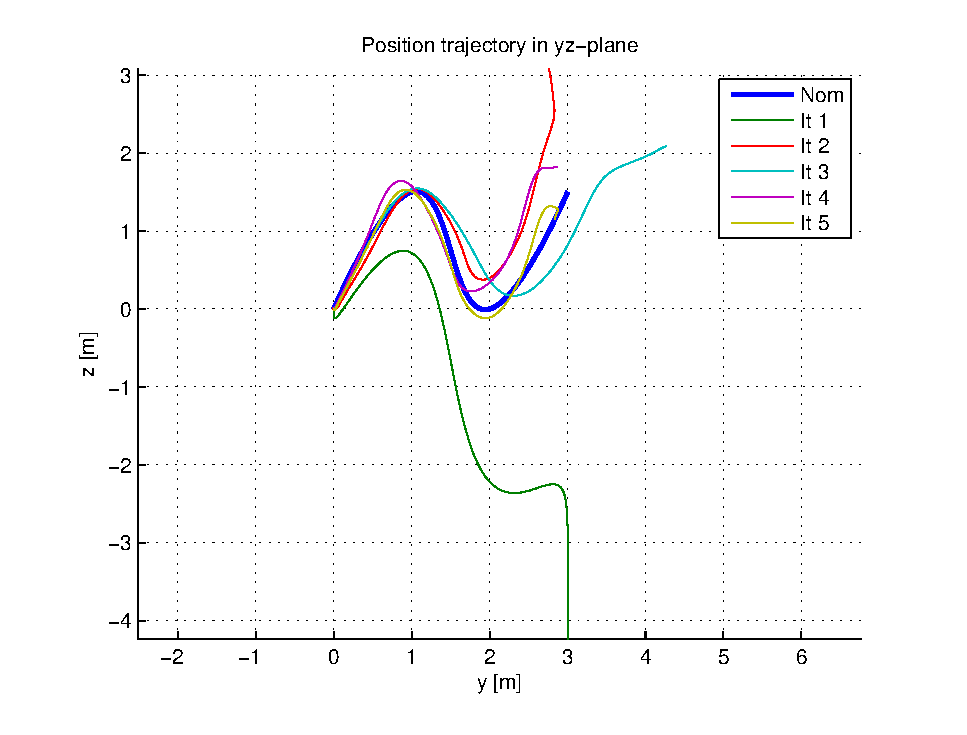
\includegraphics[scale=0.50]{ILCgravity_yz.eps}	
%\caption{Tracking results for ILC under gravity mismatch}
%\label{fig:ilc_x1}
%\end{figure}
%
%\begin{figure}
%\center
%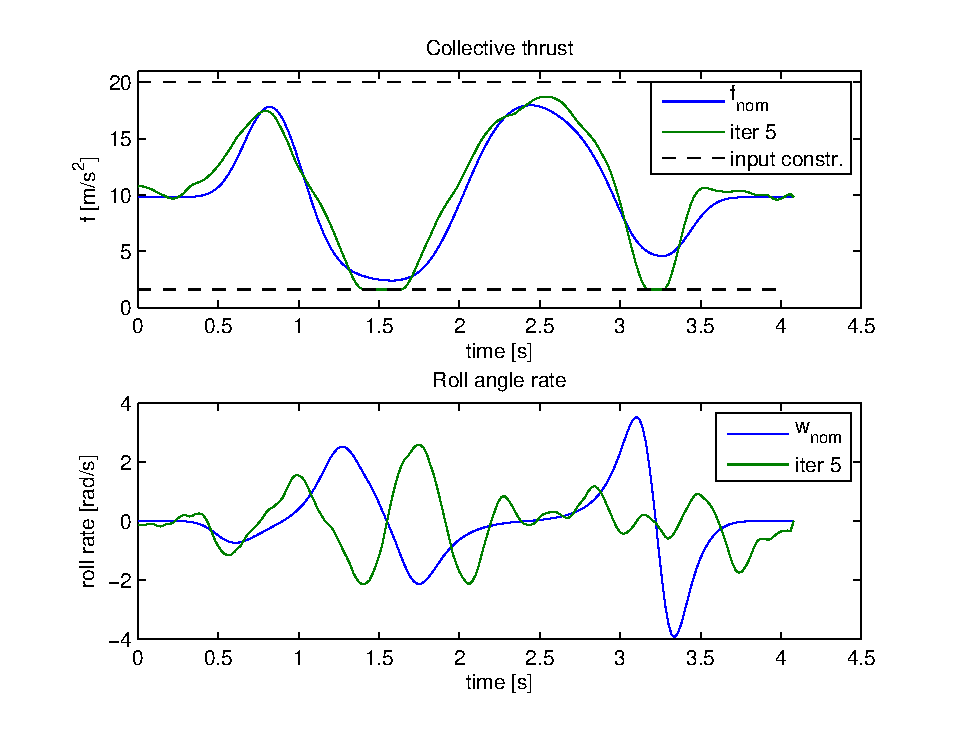
\includegraphics[scale=0.50]{ILCgravity_us.eps}	
%\caption{Control inputs over ILC iterations}
%\label{fig:ilc_u1}
%\end{figure}

%Figure \ref{fig:ilc_u1} shows the change in the control inputs needed to accommodate the gravity mismatch. Only the final input is shown, for better visibility.

Here we show the $\alg$ learning results for the quadrocopter operating under a gravity mismatch. The gravity is taken to be $g_{\mathrm{uranus}} = 10.5$, but the nominal dynamics is assuming earth gravity, $g_{\mathrm{earth}} = 9.81$. We model the cost function \eqref{QuadTheta0} as having bounded RKHS-norm, $\|\cost(\sysInput;\context)\|_{k}^{2} < B$ under the following covariance function:
\begin{align*}
k(\ctxaction, \ctxaction') &= k_u(\sysInput, \sysInput')k_{c}(\context, \context') + \sigma_{n}^{2}\delta_{aa'} \\ 
k_u(\sysInput, \sysInput') &= \sysInput^{\mathrm{T}}\Lambda_{u}^{-2}\sysInput' \\
k_{c}(\context, \context') &= \sigma_{s}^{2}\exp(-\frac{1}{2}(\context-\context')^{\mathrm{T}}\Lambda_{c}^{-2}(\context-\context'))
\end{align*}
where $\ctxaction = (\sysInput;\context)$. Diagonal matrices $\Lambda_{u}$ and $\Lambda_{c_{i}}$ transform anisotropic coordinates into isotropic coordinates or they can be motivated from Automatic Relevance Determination (ARD) point of view where $\Lambda_{u}^{2}$ and $\Lambda_{c}^{2}$ encode the relevance of inputs and contexts, respectively \cite{Rasmussen06}. The bound on the noise, $\sigma_{b}$ was set to 0.15 during the simulations.
%This general structure can be kept for all cases, where model mismatch is expected only in the drift term of the dynamics \eqref{eq:readDynamics}.

In Figure \ref{fig:comparison} we compare the performance of $\alg$ with ILC and (nonlinear) MPC with horizon $M = 5$. Weighted Sum of Squared Errors (SSE) in \eqref{costDiscrete} are plotted to show learning during the first 6 episodes. A weighted squared Euclidean distance is used as the cost function where the diagonal matrix with entries $(1,1,1,1,0.01)$ is taken as the weighting matrix $Q$. The best results for the three algorithms during the episodes are shown in Table \ref{SSE_errors}. Figure \ref{fig:comparison} clearly shows that the method can outperform more conventional methods like MPC when disturbances in the form of unknown dynamics are present, and can compare favorably with feedforward learning controllers like ILC. The yz-trajectories followed during these episodes are plotted in Figure \ref{fig:trajectories}.

\begin{figure}
\center
%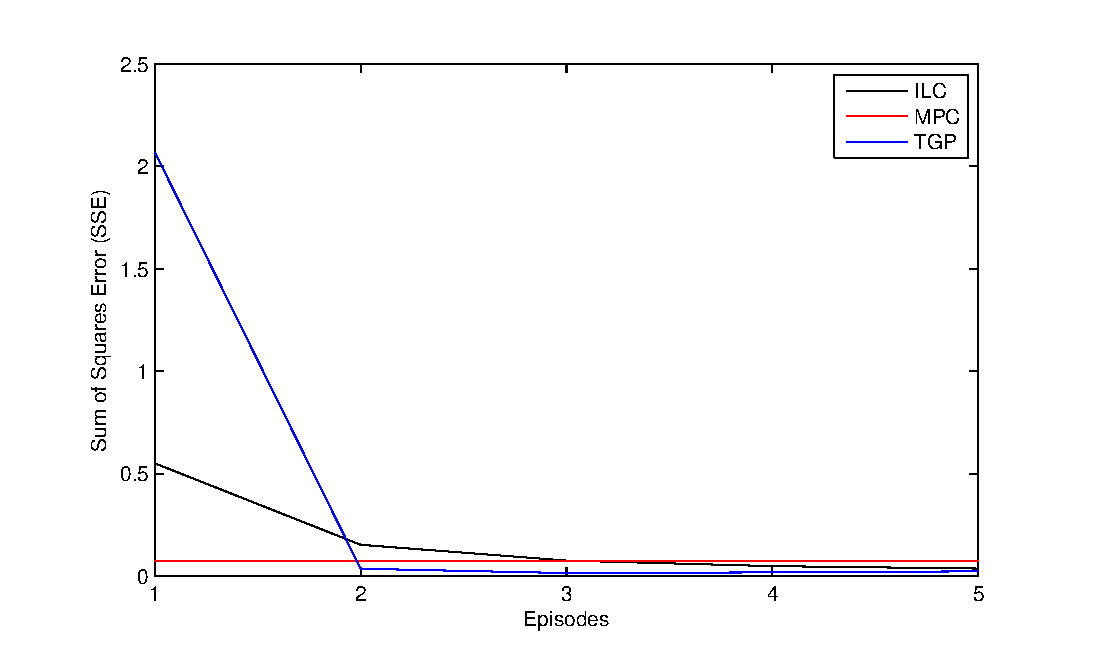
\includegraphics[scale=0.50]{comparison.eps}			
\scalebox{.5}{% This file was created by matlab2tikz v0.4.4 running on MATLAB 8.5.
% Copyright (c) 2008--2013, Nico Schlömer <nico.schloemer@gmail.com>
% All rights reserved.
% 
% The latest updates can be retrieved from
%   http://www.mathworks.com/matlabcentral/fileexchange/22022-matlab2tikz
% where you can also make suggestions and rate matlab2tikz.
% 
\begin{tikzpicture}

\begin{axis}[%
width=5.65104166666667in,
height=3.70994791666667in,
scale only axis,
separate axis lines,
every outer x axis line/.append style={darkgray!60!black},
every x tick label/.append style={font=\color{darkgray!60!black}},
xmin=1,
xmax=5,
xtick={1, 2, 3, 4, 5},
xlabel={Episodes},
every outer y axis line/.append style={darkgray!60!black},
every y tick label/.append style={font=\color{darkgray!60!black}},
ymode=log,
ymin=0.01,
ymax=10,
yminorticks=true,
ylabel={Sum of Squares Error (SSE)},
legend style={draw=black,fill=white,legend cell align=left}
]
\addplot [
color=black,
dashed,
line width=1.0pt,
forget plot
]
table[row sep=crcr]{
1 0.550705874707667\\
2 0.152998198590581\\
3 0.0758718186428609\\
4 0.0488997673400057\\
5 0.036794112098251\\
};
\addplot [
color=black,
dotted,
line width=1.0pt,
forget plot
]
table[row sep=crcr]{
1 0.0721076828940491\\
2 0.0721029920253314\\
3 0.0721240571623911\\
4 0.0721240685520741\\
5 0.0721240669971075\\
};
\addplot [
color=black,
solid,
line width=1.0pt,
forget plot
]
table[row sep=crcr]{
1 2.06972347152254\\
2 0.0360202528499323\\
3 0.0146321250277303\\
4 0.0178084331707058\\
5 0.0233960146241748\\
};
\end{axis}
\end{tikzpicture}%}
\caption{Comparison of $\alg$, ILC and MPC.}
\label{fig:comparison}
\end{figure}


\begin{figure}
\center	
% This file was created by matlab2tikz v0.4.4 running on MATLAB 8.0.
% Copyright (c) 2008--2013, Nico Schlmer <nico.schloemer@gmail.com>
% All rights reserved.
% 
% The latest updates can be retrieved from
%   http://www.mathworks.com/matlabcentral/fileexchange/22022-matlab2tikz
% where you can also make suggestions and rate matlab2tikz.
% 
\begin{tikzpicture}

\begin{axis}[%
width=0.8\columnwidth,
height=0.630967741935484\columnwidth,
scale only axis,
xmin=0,
xmax=0.3,
ymin=0,
ymax=0.35
]
\addplot [
color=blue,
dashed,
forget plot
]
table[row sep=crcr]{
-1.22568529189217e-17 1.70219232680293e-47\\
-1.22078040529282e-17 2.17466204815869e-20\\
1.24930069097586e-15 5.59329658828069e-16\\
4.31962537102899e-13 1.9152423618868e-13\\
2.51770978879146e-11 1.11631432791867e-11\\
5.55015544523879e-10 2.46106431437956e-10\\
6.60280135771012e-09 2.9283319802688e-09\\
5.12320770129383e-08 2.27281407753508e-08\\
2.90255123674167e-07 1.28827401032052e-07\\
1.29124388293531e-06 5.73511237251698e-07\\
4.73949589296885e-06 2.10713748978966e-06\\
1.48681255318932e-05 6.6189380207418e-06\\
4.09129882041033e-05 1.82444393148059e-05\\
0.000100718153544017 4.50090857862532e-05\\
0.000225245856791989 0.000100919801590805\\
0.000463240655356511 0.000208196459707293\\
0.000884823147305501 0.000399120180670242\\
0.00158255610123486 0.000716854697447387\\
0.00266870907570527 0.00121464755420377\\
0.0042680934828865 0.00195306659807664\\
0.00650682428145541 0.00299533100932766\\
0.00949841893898853 0.00440125030957139\\
0.0133294488642299 0.00622065804358311\\
0.0180472586508033 0.00848740810159894\\
0.0236519674180277 0.0112149390444555\\
0.0300941529569334 0.0143941271208937\\
0.0372785249971626 0.0179937242124732\\
0.0450728081170337 0.0219632243456565\\
0.0533202318837492 0.0262376267222215\\
0.0618536166580361 0.0307433345872289\\
0.0705090712117028 0.0354043703208843\\
0.0791376965311413 0.0401481768418987\\
0.0876142690996799 0.0449104641836341\\
0.0958424961170963 0.0496387890730672\\
0.10375696557487 0.0542947727843779\\
0.111322280599518 0.0588550337458356\\
0.118530050316482 0.06331102120878\\
0.125394431996405 0.0676679861084513\\
0.131946828905364 0.0719433270169786\\
0.138230198729659 0.0761645191587581\\
0.144293265660084 0.0803667887860157\\
0.150184789161511 0.084590646654827\\
0.155947944238694 0.0888793518508938\\
0.161614820549927 0.0932763463165637\\
0.167201052648133 0.0978226842719481\\
0.172700648861156 0.102554481146252\\
0.178081188148765 0.107500424919056\\
0.183279696817351 0.112679429291778\\
0.188199689821794 0.11809856122523\\
0.192710046988842 0.123751440482291\\
0.196646565585241 0.12961737738435\\
0.199817148084927 0.135661573700226\\
0.202011400876493 0.141836677658674\\
0.20301387722613 0.148085506344443\\
0.202619789967853 0.154344644220661\\
0.20065273345486 0.160548886433011\\
0.196983021746862 0.166636203811203\\
0.191544736744952 0.172552738672092\\
0.184349409899893 0.178257268594913\\
0.175494381526898 0.183724581129977\\
0.165164317442443 0.188947295992029\\
0.153625080784607 0.193935846625374\\
0.1412100661361 0.198716567169214\\
0.12830006671719 0.203328087323888\\
0.115298606077758 0.207816473182085\\
0.10260527646616 0.212229725482657\\
0.0905898807700316 0.216612327368361\\
0.079570030652499 0.221000508160764\\
0.0697943393352088 0.225418764413873\\
0.0614325578259062 0.229877979341309\\
0.0545730774278078 0.234375244026284\\
0.0492273137352959 0.238895250492305\\
0.0453397371877769 0.243412935431724\\
0.0428018209176867 0.247896930561529\\
0.0414679809317703 0.252313332254143\\
0.0411716730700138 0.25662933480681\\
0.0417402386729666 0.260816396765839\\
0.0430079265640447 0.264852853167071\\
0.0448258671359753 0.268725657669276\\
0.0470681659059565 0.272431034965027\\
0.0496347242551211 0.275974250701863\\
0.0524515935766653 0.279368747748684\\
0.0554695907154709 0.282634858417776\\
0.0586617700544091 0.285798252905515\\
0.0620201947143181 0.288888235420426\\
0.0655523003124128 0.291935958228636\\
0.0692770158504934 0.294972594140621\\
0.0732207080290693 0.298027491449363\\
0.0774129544020573 0.301126332090716\\
0.0818821323091202 0.304289323201106\\
0.086650838109129 0.307529473239184\\
0.0917312255322955 0.310851034404806\\
0.0971204675308709 0.314248229434997\\
0.102796687767279 0.317704416545961\\
0.108715848493778 0.321191871765943\\
0.114810181592199 0.324672370955634\\
0.120988762173356 0.328098721508834\\
0.127140705706413 0.3314173160038\\
0.133141194808927 0.33457165455712\\
0.138860120113893 0.33750661939838\\
0.14417260737948 0.340173109510588\\
0.148970203575231 0.342532494031226\\
0.15317114157554 0.344560265930261\\
0.156728025765686 0.346248311683806\\
0.159631560364095 0.347605376663323\\
0.16190957122079 0.348655584952959\\
0.163621436389131 0.349435214610502\\
0.164848937801264 0.349988255460754\\
0.165685237911466 0.350361500346063\\
0.166223974647865 0.350599977591089\\
0.166550272189824 0.350743403168433\\
0.166734851771187 0.350824053127807\\
0.166831595215191 0.350866113799758\\
0.166878121826248 0.350886259282569\\
0.166898406741448 0.350895013534916\\
0.166906302339804 0.350898412202254\\
0.16690899217171 0.35089956776726\\
0.166909773384699 0.350899902896113\\
0.166909959992641 0.350899982867216\\
0.166909994843181 0.350899997792469\\
0.166909999566499 0.350899999814467\\
0.166909999980335 0.350899999991584\\
0.166909999999663 0.350899999999856\\
0.166909999999999 0.3509\\
0.16691 0.3509\\
0.16691 0.3509\\
};
\addplot [
color=white!80!black,
solid,
forget plot
]
table[row sep=crcr]{
-1.22568529189217e-17 1.70219232680293e-47\\
0.00149999999999999 1.73668336765836e-47\\
0.00364763014665518 1.77188072066317e-47\\
0.0055173391670253 1.80768534835433e-47\\
0.00720126387170166 1.84413345781566e-47\\
0.00845435282050575 4.47782881726102e-11\\
0.00972249609462371 3.50039067992733e-10\\
0.0107264360352423 1.72575357550888e-09\\
0.0116827027554139 7.97433924187334e-09\\
0.0125142992690406 3.52969707968907e-08\\
0.0132795695984057 1.40739281842778e-07\\
0.0139891972741648 2.48780902610805e-06\\
0.0147072564012834 1.58931424439371e-05\\
0.0155933043630555 4.75467837586691e-05\\
0.0170363732779218 0.000116797459737849\\
0.0196011352333966 0.000262954307250499\\
0.0233368204789269 0.000540047820536727\\
0.0280793377847101 0.00101901903869405\\
0.0333405947757355 0.00174426548060433\\
0.039829079890062 0.00283102712170185\\
0.0457807816192392 0.00428033428663946\\
0.0514451263016625 0.00596510424689875\\
0.0582459279003183 0.00794457784762185\\
0.0656702149829863 0.0105196744040181\\
0.0734028703653534 0.0135019618069651\\
0.0810783286835201 0.016822706849945\\
0.0893912437831073 0.020547635776133\\
0.0980860842370329 0.0246153609362813\\
0.107386518532774 0.0289821778496015\\
0.116912981783451 0.0335608262331478\\
0.126250184733691 0.038263174070043\\
0.135275823376861 0.0430250257097532\\
0.144505979081848 0.0477896206311828\\
0.15460280946207 0.0524914613477293\\
0.164750098111801 0.0570938971716789\\
0.174601103433759 0.0615793527118072\\
0.183515589823985 0.0659736313716825\\
0.19136648864047 0.0702912606621299\\
0.198717131264983 0.0745394205306508\\
0.205319246465637 0.078752091960808\\
0.211634717627719 0.0829537447883885\\
0.217838130849888 0.0871813983619323\\
0.224053525033896 0.0914843587580388\\
0.230290262731955 0.0959102274984561\\
0.236493339715277 0.10049371072813\\
0.242589736117166 0.105270439487442\\
0.248511406568802 0.110266204278065\\
0.254189545914904 0.11549714013692\\
0.259533973423337 0.12096814049853\\
0.264419606172869 0.126670920100997\\
0.268689538314935 0.132582978575214\\
0.272150708907525 0.138667235880877\\
0.274561071344487 0.14487314244445\\
0.275673002191072 0.151141662345644\\
0.275713816705104 0.157404476271074\\
0.276883680675954 0.163447726433572\\
0.277760942123325 0.16918446319552\\
0.27824265781471 0.174073522101255\\
0.278149263497095 0.177526626998138\\
0.274485324428871 0.180895637488242\\
0.267260571601381 0.18428842690175\\
0.25753673904649 0.187939359894377\\
0.246417649110064 0.192390105012675\\
0.234348830191734 0.197059905025091\\
0.221856585787478 0.201551782713903\\
0.209486761545213 0.205944642060925\\
0.197728451288954 0.210322962934804\\
0.186956399809314 0.214712625588846\\
0.17742607857495 0.219135164717393\\
0.169293237592045 0.223599838887261\\
0.162633443760857 0.228104333263364\\
0.157461810340823 0.232626698513717\\
0.153750655159289 0.237144816349716\\
0.15144065258976 0.241625873648307\\
0.150438402287753 0.246034913616617\\
0.150604446746411 0.250337569224309\\
0.151749540098945 0.25450053462317\\
0.153654407686669 0.258506688710851\\
0.156102764949529 0.262345943869841\\
0.158909186064691 0.266017573934853\\
0.161931663283745 0.269530993585847\\
0.165075856447712 0.272900858575368\\
0.168296096344847 0.276146310428268\\
0.171589228231251 0.279297596563365\\
0.174983035587055 0.282380608542136\\
0.178523731744706 0.285424835112467\\
0.182264244478577 0.288461783872536\\
0.186253420940537 0.291521369471758\\
0.190527476934042 0.294624917372156\\
0.195106052929824 0.297791676253693\\
0.199992421595481 0.301038469014114\\
0.205174980279097 0.304369684182669\\
0.210628683744048 0.307776406523703\\
0.216319015460516 0.31124227028071\\
0.222211024147843 0.314732878342914\\
0.228280194618683 0.318211192636775\\
0.23452671032221 0.32163428168387\\
0.241002111330529 0.324934195587954\\
0.247771041405099 0.328039525226392\\
0.254725798922942 0.330879536056328\\
0.261670924145881 0.333394165632125\\
0.268449109784845 0.335544699640135\\
0.274600109781586 0.337345247128335\\
0.279742099108407 0.338829205500537\\
0.283797618649932 0.340026006438742\\
0.286896403439546 0.340956566043168\\
0.289262824392623 0.341648334994253\\
0.290943353992031 0.342142161410553\\
0.29202188826538 0.342476982441897\\
0.292649373042531 0.34269148819576\\
0.292977936068079 0.342823656882954\\
0.293122703585512 0.342898406732506\\
0.293161966504658 0.342937912935062\\
0.293144511184251 0.342959973411522\\
0.293098009447051 0.342969176743278\\
0.293036858361144 0.342972950725491\\
0.292965794423808 0.342975154709904\\
0.292890031933476 0.342978238710967\\
0.292812761427382 0.342982771956726\\
0.292732200136343 0.342984396915278\\
0.292649587685881 0.342985900905412\\
0.292564033026197 0.342989145326842\\
0.292474712590903 0.342990606410152\\
0.292382693155756 0.342992227666699\\
0.292287998585562 0.342995794408036\\
0.292190694783464 0.342997328741063\\
};
\addplot [
color=white!70!black,
solid,
forget plot
]
table[row sep=crcr]{
-1.22568529189217e-17 1.70219232680293e-47\\
-6.96894886532803e-05 6.7068747997345e-07\\
-0.000202839376588429 3.34138048794965e-06\\
-0.0003280087283286 3.81643411414663e-06\\
-0.000449675745049249 4.51398900574061e-06\\
-0.000570002283619798 7.63071642349851e-06\\
-0.000690467517474069 8.32379866221699e-06\\
-0.000810847313375079 9.03047236403291e-06\\
-0.00093100811316666 1.17171733950413e-05\\
-0.00105041372887553 1.58425130692391e-05\\
-0.00116741338358483 1.80716691384592e-05\\
-0.00127658087826819 2.33589926852617e-05\\
-0.00136604439173597 3.86292756529383e-05\\
-0.0014112272852817 6.92756992517406e-05\\
-0.00136551285130495 0.00012554957631895\\
-0.00115000889697326 0.000237185247754649\\
-0.000652688781023135 0.000437533493525421\\
0.000246315421877469 0.000772318915290228\\
0.00163818330540071 0.00129702769395246\\
0.00359626911628759 0.00207142744746206\\
0.00625110016190025 0.0031636489419408\\
0.00982209327278499 0.00463984056971599\\
0.0144775641772967 0.00655830260263772\\
0.0201482582783218 0.00894146236961583\\
0.0265906848538277 0.0117810911808025\\
0.0336039899634732 0.0150441430249942\\
0.0411170581868269 0.0187081136923171\\
0.0491392257184986 0.0227415093636831\\
0.0576088843094974 0.0270561589183701\\
0.0663111845775567 0.0315904288931203\\
0.0750036381942423 0.0362682701349964\\
0.0835457135615783 0.0410177184291957\\
0.0918967737804798 0.0457821211611094\\
0.100038953815395 0.0505098759803383\\
0.107929127474172 0.0551596306101606\\
0.115508500414759 0.0597096957138572\\
0.122728566033978 0.064154203625479\\
0.129569645840951 0.068500798001233\\
0.136048480014242 0.0727684028350492\\
0.14221703967537 0.0769841486356765\\
0.148155887018902 0.0811816266279981\\
0.153959612825991 0.0854063176674784\\
0.159709444931955 0.0897004162769665\\
0.165444948251009 0.0941066065953106\\
0.171157074371238 0.0986712307988215\\
0.176803423921076 0.103427854006391\\
0.18232375988143 0.108403099318434\\
0.187642892061035 0.113613703324282\\
0.192662055535353 0.119067580980374\\
0.197251075527947 0.124752373247577\\
0.201244875475475 0.130647136457809\\
0.204439082550951 0.136716955369744\\
0.206588927226967 0.14291159776564\\
0.20745549482893 0.149172501381595\\
0.206915074253492 0.15543646196156\\
0.204993483637013 0.161630979205183\\
0.201650105601112 0.167680434434504\\
0.196866178071567 0.173512710265168\\
0.190664183117823 0.179084307285456\\
0.182681722518448 0.184417578995579\\
0.172898042829906 0.189532483181641\\
0.161796155514204 0.194432029443228\\
0.14969206429371 0.199152444542122\\
0.136919763836693 0.203731346630123\\
0.123920993809732 0.208206974944566\\
0.111162107111837 0.212614144545703\\
0.0990625742601031 0.216994517118333\\
0.0879642268657965 0.22138262960088\\
0.0781170255366198 0.225802102387589\\
0.0696804839918491 0.230263038524489\\
0.0627324939176528 0.234761761368155\\
0.0572816425030556 0.239283095722647\\
0.0532816348511079 0.243802699354131\\
0.0506433031039171 0.248284819132488\\
0.0492432509689337 0.252697482799736\\
0.0489315043252583 0.257006114313992\\
0.0495394802004452 0.261180285175043\\
0.0508901760124632 0.265202884062001\\
0.0528109985160834 0.26905926260632\\
0.055147438978943 0.27274756151488\\
0.0577738821264097 0.27627493237729\\
0.0606002037729684 0.2796551160931\\
0.0635729441719989 0.282907485153931\\
0.0666719144838178 0.286062965535056\\
0.0699029243689663 0.289148230855588\\
0.0732911815026782 0.292193368300783\\
0.0768743757555208 0.295230187382803\\
0.0806939626586606 0.298288573695643\\
0.0847862750776853 0.301389737801274\\
0.0891762248813187 0.30455484844913\\
0.0938751934008776 0.307801152330588\\
0.0988804836846788 0.311128007424248\\
0.104174012507083 0.314528691233995\\
0.109724184460128 0.317987909594139\\
0.115490965477274 0.321476787192024\\
0.121431417382486 0.324956570358377\\
0.127502293951523 0.328378827231132\\
0.13366916603205 0.331686871001775\\
0.139891322706114 0.334818375814156\\
0.146032063559 0.337707389541212\\
0.151928000077407 0.340302392014691\\
0.157555378674008 0.342553127419426\\
0.162770092027016 0.344445841143984\\
0.167205402034419 0.346003129334002\\
0.170695051007873 0.347258012857838\\
0.173370075677522 0.348228335471384\\
0.175384372524899 0.348948023807221\\
0.176794059304187 0.349459113677153\\
0.177670106411552 0.349803570089982\\
0.178146951720567 0.350024087099772\\
0.178355275547524 0.350161262846089\\
0.178393874709006 0.350237715248448\\
0.178332384034663 0.35027686757289\\
0.178216268578435 0.350296100757662\\
0.178072533327515 0.350306763401324\\
0.177915794147076 0.350310290003338\\
0.177753312333561 0.350312303315011\\
0.177588247940206 0.350316790642978\\
0.177421817716019 0.350317731406291\\
0.17725449623045 0.350317741137956\\
0.17708638234394 0.350317772169235\\
0.176917476048034 0.350317535886859\\
0.176747777314441 0.350316743677559\\
0.176577286095035 0.350315106928069\\
0.176406002321851 0.350312337025129\\
0.176234346726264 0.350308423644074\\
};
\addplot [
color=lightgray!80!black,
solid,
forget plot
]
table[row sep=crcr]{
-1.22568529189217e-17 1.70219232680293e-47\\
-0.000102568949184313 2.14605271233367e-07\\
-0.000303788531108529 1.74857617570992e-06\\
-0.000499888804145477 4.56482952616162e-06\\
-0.000694258789205412 4.51247981153966e-06\\
-0.000887396777818861 2.25668808317227e-06\\
-0.00107960068965544 2.06519083109562e-06\\
-0.00127134047264853 3.03857541779534e-06\\
-0.00146261594802475 2.74632664200539e-06\\
-0.00165255839739505 6.36865016343942e-07\\
-0.00183914878882561 1.76870721426562e-06\\
-0.0020177458834021 5.84322812667045e-06\\
-0.00217745569589737 1.51140919261623e-05\\
-0.00229635423772238 4.23813470069488e-05\\
-0.0023341032548636 0.000100297648208137\\
-0.00222416095366973 0.000211169045398321\\
-0.00187206356655781 0.000408667419953657\\
-0.00116869731257434 0.000737902071052488\\
-1.14024163137031e-05 0.00125323200071849\\
0.00169305200396138 0.00201416669641234\\
0.00406025762584899 0.00308789083725242\\
0.00726126718418169 0.00453680012361265\\
0.0114636786176171 0.00641834287593941\\
0.0166845077654631 0.00876150935985416\\
0.0227601118670432 0.0115672784628738\\
0.0295018606249058 0.0148054423556164\\
0.0368146348786742 0.0184453600443373\\
0.0446627401170529 0.0224477626473323\\
0.0529520248834549 0.0267499611306068\\
0.0614887343129075 0.0312762917974416\\
0.0700619682218682 0.0359501452114404\\
0.0785264202082638 0.0407015145310686\\
0.0868103228714343 0.0454669432480147\\
0.094867627174318 0.0501940219409489\\
0.102647581620648 0.0548453418825652\\
0.110102765095429 0.0593984474881154\\
0.117202080388081 0.0638462559721728\\
0.123939330964828 0.0681956794469533\\
0.130336299211738 0.0724652555016672\\
0.136440138174559 0.0766821675207179\\
0.142318588179577 0.0808801496874782\\
0.148050342651082 0.0851045823054236\\
0.153704354559034 0.0893972673447128\\
0.159318123664425 0.0938004411125134\\
0.164892107141419 0.0983601556932665\\
0.170397820352984 0.103110447500443\\
0.175784343178216 0.108078598698901\\
0.180978838587374 0.113282044742766\\
0.185881571490875 0.118728979954117\\
0.190361081146273 0.12440700337141\\
0.194251102749291 0.13029527068154\\
0.19734927819964 0.136359658910645\\
0.199420450876635 0.142550468297902\\
0.200232056736069 0.14880917293248\\
0.199633268483391 0.155072301419226\\
0.197578322443034 0.161270626275162\\
0.193996276365486 0.167335733514658\\
0.188837316271466 0.173198726858659\\
0.182164954175845 0.17880864502373\\
0.173814990950176 0.184173828471407\\
0.16377026933587 0.189312788378253\\
0.152430799445364 0.194235272599214\\
0.140135925826028 0.19897140877519\\
0.127223210228555 0.203558201875177\\
0.114129398530379 0.208035849612539\\
0.101299672729903 0.212444770197069\\
0.0891345675283825 0.216827899733808\\
0.0779675311823171 0.221215816495472\\
0.0680483417451137 0.225634295656912\\
0.0595395849775893 0.230094729240571\\
0.0525221215979611 0.234592957694269\\
0.0470053690248887 0.239113420355176\\
0.0429400731185863 0.243631443267651\\
0.0402307052903308 0.248116428992566\\
0.0387461239498512 0.2525300824077\\
0.0383308361572524 0.256841381446586\\
0.0388161436961861 0.26102061084043\\
0.0400312041407295 0.265045268292501\\
0.0418136449185453 0.268906764413183\\
0.0440186018751067 0.272600472185914\\
0.0465282885774816 0.276129370132768\\
0.0492572956942079 0.279513378479327\\
0.0521525126971491 0.282771594698441\\
0.0551904833859881 0.285928639772023\\
0.0583714107212857 0.289012603164623\\
0.0617141785856946 0.29205781144256\\
0.0652506700732569 0.295093484343511\\
0.0690185302701033 0.298147447880141\\
0.0730528381048807 0.301247612543005\\
0.077379807387317 0.304416488698925\\
0.0820141527053808 0.307659747843176\\
0.0869568416614227 0.310979495676232\\
0.0921934091779344 0.314376535615258\\
0.0976942175085982 0.317834941646647\\
0.103418025559389 0.32132345308338\\
0.109315368012795 0.324803069365504\\
0.11532813638267 0.328226020070213\\
0.121397128726327 0.331536639522886\\
0.127459054072022 0.334674536600388\\
0.133376999110381 0.3375761268522\\
0.138981069838758 0.340191988440471\\
0.144230234313236 0.342474621176746\\
0.149052665038748 0.344404295358724\\
0.153174984920509 0.345993917794497\\
0.156431524669876 0.34727380304348\\
0.158924878194692 0.34826412339362\\
0.160790962542958 0.34899606414335\\
0.162082728558974 0.349513445830185\\
0.162872801594043 0.349865154564198\\
0.163288663070431 0.350091372034434\\
0.163450551449463 0.350227532241392\\
0.163449542200114 0.350303979732393\\
0.16335099059564 0.350344442263634\\
0.16319851657109 0.350366483645559\\
0.16301858003668 0.350375173048677\\
0.162825811521144 0.350378158734582\\
0.162625206483452 0.350379502158031\\
0.162422438776467 0.350381544504493\\
0.16222107229239 0.350384849148572\\
0.16201899949556 0.350388224653819\\
0.161816220441376 0.350390131291591\\
0.16161343513676 0.350389143491773\\
0.161410551538701 0.350385174105608\\
0.16120677845556 0.350381767471496\\
0.161002906039375 0.35038165357792\\
0.160799312123579 0.350381879534353\\
};
\addplot [
color=gray!80!black,
solid,
forget plot
]
table[row sep=crcr]{
-1.22568529189217e-17 1.70219232680293e-47\\
-0.000114512356556703 1.25127393446594e-07\\
-0.00034070276508775 1.02242857021055e-06\\
-0.000561226236775428 3.46095750199662e-06\\
-0.000780296465662392 6.87092518825578e-06\\
-0.00100032265189235 7.4652816482698e-06\\
-0.00121984141163884 8.24945243468973e-06\\
-0.00143878419850366 1.15613887706163e-05\\
-0.00165686859892804 1.23471487581013e-05\\
-0.00187359210967526 1.36724200386783e-05\\
-0.00208722374857171 1.87442096209344e-05\\
-0.00229314650295718 2.41676853887233e-05\\
-0.00248068653661868 3.6612326012786e-05\\
-0.00262889749165903 6.59225754487153e-05\\
-0.00269982956653407 0.00012431523207416\\
-0.0026318209791874 0.00023399159320517\\
-0.00233730405016909 0.000427352049705375\\
-0.0017126167315161 0.000753918952540572\\
-0.000651435736079118 0.00126569189014515\\
0.000949803751899945 0.00202390206102909\\
0.0032052821264139 0.00309251078912576\\
0.00626471185566026 0.00452998443130141\\
0.0102812194968579 0.00639296620316021\\
0.0152960855667051 0.00871749999530171\\
0.0211892924450988 0.0115036584556266\\
0.0277928039075072 0.0147296069700197\\
0.0350053126914217 0.018363093119388\\
0.0427694111800621 0.0223590123435033\\
0.0509748247471717 0.026655632697963\\
0.0594357346245813 0.0311780319669186\\
0.0679552229725003 0.0358491126380794\\
0.076385865184333 0.0405976474678303\\
0.0846423988001716 0.0453600734545225\\
0.0926664724986964 0.0500862847182066\\
0.100403307800579 0.054736396731311\\
0.107809161851591 0.0592893631577414\\
0.114859677875729 0.0637352099806183\\
0.121554506876615 0.0680851529090404\\
0.127917717160198 0.0723566936124065\\
0.133994570571656 0.0765751472983688\\
0.139847392337793 0.0807759596610802\\
0.145547756911404 0.0849993630064979\\
0.151158624775579 0.0892924510044185\\
0.156715601975193 0.0936999435138078\\
0.162223036454036 0.0982576181915653\\
0.167659132184213 0.103000730231796\\
0.172977960483689 0.107961603485793\\
0.178108352716742 0.113159913858699\\
0.182950590900196 0.118600612269306\\
0.187372264295425 0.12427760012343\\
0.191207092744037 0.130164861130671\\
0.194254592548235 0.136228002475708\\
0.196285641176356 0.142417451056541\\
0.197071229999883 0.148675358350079\\
0.196447749429693 0.154938135065333\\
0.194337908475433 0.161137366445786\\
0.190658159785757 0.16720638191571\\
0.185347711830382 0.173080946032874\\
0.178467722569003 0.178712411306817\\
0.1699336995313 0.184097249078138\\
0.159761129404468 0.189251054666783\\
0.148313238250394 0.194183907820215\\
0.13592962552207 0.198923573400382\\
0.122953952264081 0.203512705307245\\
0.109818603427338 0.207990644048298\\
0.0969581733976403 0.212399174258475\\
0.0847646219909961 0.216780129501278\\
0.073567260461676 0.221168196407479\\
0.0636156730474405 0.225587143045511\\
0.055074023000827 0.230047299781676\\
0.0480248261950877 0.234545339726147\\
0.042478042219663 0.239065683949415\\
0.0383832610794527 0.243583699949907\\
0.035642193680292 0.248068835632912\\
0.0341202011995601 0.25248295433325\\
0.0336588167372602 0.256796016755185\\
0.0340886091432951 0.260980377372318\\
0.035241241835521 0.265008984264384\\
0.036958726876154 0.268872395512835\\
0.0391010840361433 0.272567764796139\\
0.0415544527763854 0.276100529787375\\
0.0442356037859225 0.279483451799353\\
0.0470925585610098 0.282742333338558\\
0.0501005336838028 0.285900825894974\\
0.0532571180934691 0.288987148769493\\
0.0565778675007659 0.292031062747608\\
0.0600919741784477 0.295063839893598\\
0.0638349368586362 0.298119123888693\\
0.0678407837458704 0.301219615997209\\
0.0721363772015091 0.30438506742319\\
0.0767378247723716 0.307630953194699\\
0.081650372801594 0.310955598029417\\
0.0868597417693063 0.31435275290488\\
0.0923355152091296 0.317811077447338\\
0.0980377383478918 0.32129988685603\\
0.103913502960727 0.324781049053622\\
0.109897339187289 0.328204999670081\\
0.115917448304014 0.331517734450258\\
0.121899072858157 0.334655604225478\\
0.127707542298521 0.337560121347124\\
0.133173563978366 0.340186705946673\\
0.138241090759914 0.342489822137843\\
0.142857696019564 0.344440190885546\\
0.146804122475456 0.346048928184029\\
0.149929905617852 0.347339064302016\\
0.1523214107822 0.348326152994448\\
0.15410416597674 0.349060880516076\\
0.15532965504223 0.349584609636619\\
0.156072419364902 0.349940128649385\\
0.156455599174936 0.350169697265851\\
0.156593231358796 0.350307198188544\\
0.156571955377746 0.3503841049599\\
0.156454622565637 0.350424758397993\\
0.156283773068867 0.350446815913649\\
0.156085519330756 0.35045555211865\\
0.155874426494805 0.350459368962191\\
0.155657904947441 0.35046354132232\\
0.155439318250402 0.350464522761915\\
0.155219847340594 0.350464561040156\\
0.15499972268927 0.350464357331647\\
0.154778945010748 0.350463636869048\\
0.154557515398803 0.350462124911597\\
0.15433543532908 0.350459546763548\\
0.154114123492652 0.350455750212026\\
0.153893525344339 0.350452045850647\\
0.153672814787058 0.350452000448613\\
};
\addplot [
color=darkgray!80!black,
solid,
forget plot
]
table[row sep=crcr]{
-1.22568529189217e-17 1.70219232680293e-47\\
-0.000120784200296735 -6.49745756573323e-07\\
-0.000360130323330247 -3.27306106458941e-06\\
-0.000596537311130501 -3.80019419459244e-06\\
-0.00083151056169772 -4.55162142197078e-06\\
-0.00106567677625733 -7.63953708668375e-06\\
-0.00129927122928073 -8.09686028967402e-06\\
-0.00153190251830635 -7.82325993047913e-06\\
-0.00176436639865595 -1.00106838467604e-05\\
-0.00199603204553688 -1.37900055651847e-05\\
-0.00222438149513322 -1.68279452814376e-05\\
-0.00244504042837358 -1.52663300623744e-05\\
-0.0026476695893667 -4.82450491215575e-06\\
-0.00281180586576328 2.10876039384351e-05\\
-0.00290081662563242 7.81428849566882e-05\\
-0.00285547623941617 0.000187518611761666\\
-0.00259218833738774 0.000382398582011791\\
-0.00201003001125025 0.000704893209241307\\
-0.00100153585169048 0.00121452317955225\\
0.000542677915865329 0.00196954306730744\\
0.00273761128349881 0.00303311146676768\\
0.00572126721128348 0.00446764189656685\\
0.00963616179600356 0.00632366791812721\\
0.0145330088390893 0.00863775975971662\\
0.0203171674323868 0.0114140628861437\\
0.0268367847084296 0.0146328273911961\\
0.0339888649427312 0.0182610706669647\\
0.0417031113324128 0.0222530748286905\\
0.0498595753461654 0.0265464168233619\\
0.0582762347328019 0.0310670613915368\\
0.0667641946390508 0.0357396177333608\\
0.0751755958376384 0.0404884230822487\\
0.0834170395974538 0.0452514037250278\\
0.0914230490698097 0.0499758919905831\\
0.0991365866264871 0.0546271470087564\\
0.106515660931593 0.0591799591097474\\
0.113539505629269 0.0636283867888796\\
0.120210829184461 0.0679761974945176\\
0.126555307560295 0.0722469570315189\\
0.132617192431507 0.0764693160121669\\
0.138455746128118 0.0806739269015211\\
0.14413834695011 0.0848988277518319\\
0.149724340639014 0.0891882643600483\\
0.155248235831181 0.0935915318775323\\
0.160718973019438 0.0981481642396253\\
0.166115491381849 0.102893641426784\\
0.171392463581888 0.107858009106762\\
0.176483262266639 0.113054446023272\\
0.181288036409203 0.118489917083899\\
0.185673809999776 0.124163004960744\\
0.189474182801642 0.130047984505528\\
0.192490170035159 0.136109696612077\\
0.194496618594321 0.142298035472598\\
0.1952667833079 0.148555099127307\\
0.194629465090535 0.154817196658235\\
0.192489000547984 0.16101655039033\\
0.188754441460266 0.167087410723659\\
0.183360286135814 0.172966625353997\\
0.17636255838275 0.178605864619596\\
0.16771817442169 0.183998361425835\\
0.157468480329916 0.189158017411451\\
0.145957110521931 0.194096072298564\\
0.133521388722181 0.19884261265979\\
0.120509710727598 0.203437489400203\\
0.107351201830433 0.20791627553909\\
0.0944737846806849 0.212322282407367\\
0.0822642372304304 0.216703600163952\\
0.0710496555399977 0.221092144253544\\
0.0610794705503767 0.225512643237304\\
0.0525188324121665 0.229972785083252\\
0.0454512772671009 0.234471531639707\\
0.0398871745481081 0.238992080874756\\
0.0357754730127481 0.243510759521878\\
0.0330162196399394 0.24799293888534\\
0.031472824302537 0.252404545511381\\
0.030985186146382 0.256717512454444\\
0.031383463381143 0.2608997580102\\
0.0325003015342248 0.264928842038301\\
0.0341797155428252 0.268790708876423\\
0.0362851649947088 0.272487118665694\\
0.0387051284677414 0.276021816881095\\
0.0413579020305276 0.279408869250073\\
0.0441919284208281 0.282668416778682\\
0.0471818050626981 0.285824885092248\\
0.0503239043715822 0.288913086585664\\
0.0536318447944696 0.291965710742531\\
0.0571326718224098 0.295002896535995\\
0.0608606987748896 0.298058312924527\\
0.0648494473948124 0.301159595490626\\
0.0691259346125197 0.304328080487282\\
0.0737074332714329 0.30757120604291\\
0.0785997658133269 0.310894540594184\\
0.0837905307873555 0.314297530377037\\
0.0892510321498635 0.317756151145921\\
0.0949402839404015 0.321244258788698\\
0.100803130436297 0.324724086702584\\
0.106769472730125 0.328147635269147\\
0.112759747774968 0.331460224866096\\
0.118692391687362 0.334602936180666\\
0.124434890275106 0.337514106984106\\
0.129819285839327 0.340146251402218\\
0.134779089471069 0.342456858622059\\
0.139268765345743 0.344418593554173\\
0.143102032156633 0.346038558150716\\
0.146144764801784 0.347339942824747\\
0.14847327164883 0.34834530949421\\
0.150202086263628 0.349087557649666\\
0.151384366113488 0.349610900164482\\
0.152096962780477 0.349966698688136\\
0.152459578925004 0.350195610925785\\
0.152582220982306 0.350334788496313\\
0.152548541086708 0.350412367347645\\
0.152419796965049 0.350452792124612\\
0.152237788413436 0.350472538081904\\
0.152028417042669 0.350483295552461\\
0.151806232276687 0.350486942073236\\
0.151578664955848 0.350488611636923\\
0.151349051176528 0.350491469089236\\
0.15111875716823 0.350491946672748\\
0.150888219132607 0.350491913665587\\
0.150657525453229 0.350493507463917\\
0.150426711923391 0.350493738601499\\
0.150195725938216 0.350493191505343\\
0.149964567425491 0.350493745418546\\
0.149733420104656 0.350495908743066\\
0.149502329355025 0.350496355129054\\
};
\end{axis}
\end{tikzpicture}%
\caption{Trajectories $\{(y_t,z_t)\}$ followed by a quadrotor under $\alg$, ILC and MPC: the dashed lines represent the trajectory that needs to be tracked. Solid lines represent the trajectories of the quadrotor tracked by the algorithms. Darker shades of gray represent increasing episodes.}
\label{fig:trajectories}
\end{figure}

\begin{table}[h!t]
% increase table row spacing, adjust to taste
\renewcommand{\arraystretch}{1.3}
\caption{SSE errors}
\label{SSE_errors}
\centering
\begin{tabular}{cc}
\textbf{Method / Episode No.} & SSE \\
\hline
MPC, horizon = 5 & 0.0617 \\
ILC, episode 6 & 0.0306 \\
TGP, episode 6 & 0.0271 \\
\end{tabular}
\end{table}

\subsection{Transfer Learning}

Here we show the transfer learning performance of $\alg$. We implement the scenario considered in section \ref{t-learning} three times using three random wave trajectories: we first run $\alg$ on an initial fixed wave trajectory $\Traj_{0}$ and then switch to a different trajectory $\Traj_{i}$, $i\in{1,2,3}$. Figure \ref{fig:tlearning} shows the tracking error of $\Traj_{i}$ under the transfer learning setting. We compare with TGP running with no prior knowledge and with ILC.

\begin{figure}
\center
%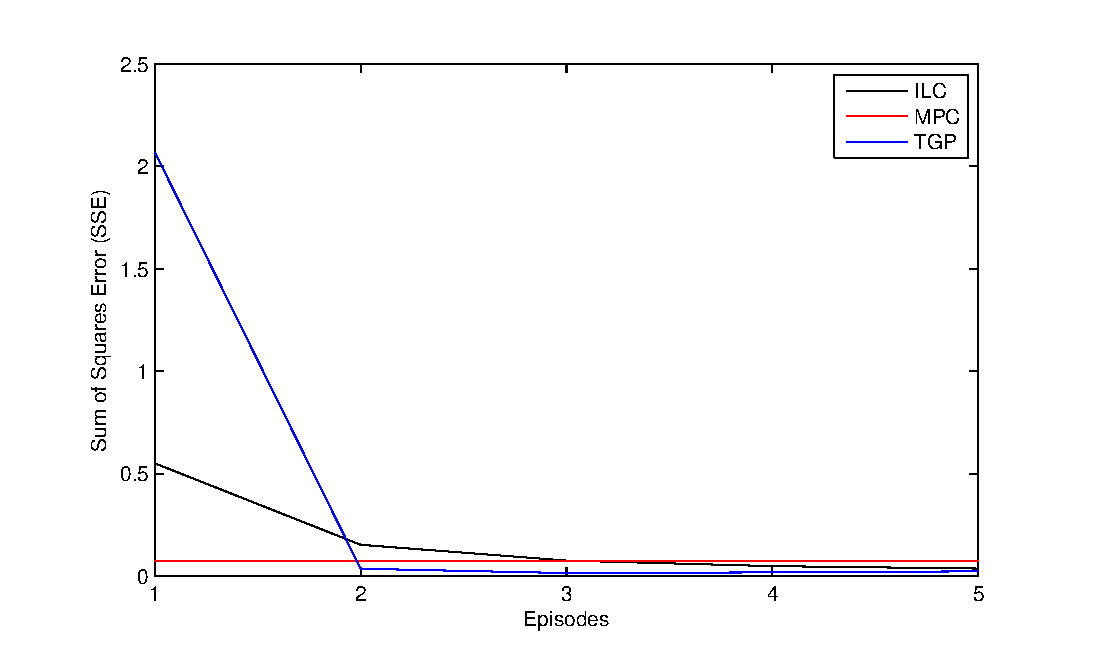
\includegraphics[scale=0.50]{comparison.eps}			
% This file was created by matlab2tikz v0.4.4 running on MATLAB 8.0.
% Copyright (c) 2008--2013, Nico Schlmer <nico.schloemer@gmail.com>
% All rights reserved.
% 
% The latest updates can be retrieved from
%   http://www.mathworks.com/matlabcentral/fileexchange/22022-matlab2tikz
% where you can also make suggestions and rate matlab2tikz.
% 
\begin{tikzpicture}

\begin{axis}[%
width=0.85\columnwidth,
height=0.670403225806452\columnwidth,
area legend,
scale only axis,
xmin=0.5,
xmax=3.5,
xtick={1, 2, 3},
xlabel={Trajectory Index},
ymin=0,
ymax=4,
ylabel={SSE - Episode 1},
legend style={at={(0.03,0.97)},anchor=north west,draw=black,fill=white,legend cell align=left}
]
\addplot[ybar,bar width=0.0503703703703704\columnwidth,bar shift=-0.062962962962963\columnwidth,draw=black,fill=white] plot coordinates{(1,0.534257)
(2,2.211294)
(3,2.305692)};

\addlegendentry{ILC};

\addplot [
color=black,
solid,
forget plot
]
table[row sep=crcr]{
0.5 0\\
3.5 0\\
};
\addplot[ybar,bar width=0.0503703703703704\columnwidth,draw=black,fill=lightgray] plot coordinates{(1,2.552392)
(2,3.56266)
(3,3.837903)};

\addlegendentry{TGP};

\addplot[ybar,bar width=0.0503703703703704\columnwidth,bar shift=0.0629629629629629\columnwidth,draw=black,fill=gray] plot coordinates{(1,0.222369)
(2,1.007975)
(3,0.543684)};

\addlegendentry{TGP-with transfer};

\end{axis}
\end{tikzpicture}%
\caption{Comparison of ILC, $\alg$ with and without transfer (from scratch). In the case of \emph{$\alg$ with transfer} the algorithm was first run on a different trajectory.}
\label{fig:tlearning}
\end{figure}


% % % % % % put more plots here % % % % % %
\section{Conclusion}\label{sec:conclusion}
In this paper, we have proposed and analyzed $\alg$, a GP-optimization based RL-algorithm, demonstrating its effectiveness in learning unknown dynamics and knowledge transfer between different contexts. We have validated its performance in numerical examples. Unknown dynamics, if severe, can prevent more conventional methods such as Model Predictive Control or Iterative Learning Control from tracking any given trajectory. $\alg$ on the other hand learns to track online a scalar cost function, and converges to a given trajectory under mild assumptions. It works by solving the exploration-exploitation problem: it \emph{explores} new control inputs when the uncertainty of that input is high enough, and it \emph{exploits} the learned dynamics as it gets better at predicting the cost function.

The sublinear regret proofs presented in \citet{Srinivas09} and \citet{Krause11} hold only when the hyperparameters of the GP from which the function to be optimized is drawn are known. In practice estimation of hyperparameters can be performed using Maximum Likelihood and its variants but we are currently unaware of any results on the sensitivity analysis. We have evidence to believe that under mild mismatch only the speed of convergence is affected, however changes in the kernel structure can hinder learning. This leads to the problem of adaptive estimation of the covariance functions \cite{Ginsbourger08}, which will play an increasing role in learning under unpredictable environments, such as those studied in RoboEarth \cite{Waibel11}.

%Theorem \ref{theorem1} and Proposition \ref{Proposition2} depend on the sublinear cumulative regret of CGP-UCB. More could be said about the stochastic convergence if the distribution of cumulative regret were known. The transfer learning gain in \eqref{transfer-learning} can also be calculated in this way. Extreme Value Theory is needed to investigate the distribution of the maximum of a Gaussian Process under different kernels. Results in \cite{McCormick00} and \cite{James07} indicate that the mean and the maximum of a Gaussian Process are asymptotically independent and that the maximum follows the \emph{Gumbel} distribution as a limiting distribution in certain cases.

%\section*{Acknowledgment}
%
% Acknowledgements should only appear in the accepted version. 
%\textbf{Do not} include acknowledgements in the initial version of
%the paper submitted for blind review.


% In the unusual situation where you want a paper to appear in the
% references without citing it in the main text, use \nocite
%\nocite{langley00}

\bibliography{cgpucb-dynsys}
\bibliographystyle{icml2014}

\appendix

\section{Proof of Proposition \ref{Proposition2}}

To prove proposition \ref{Proposition2} we start with the following lemma:
\begin{lem}
$\forall \epsilon > 0 \ \exists \ \alpha_0(\epsilon, d) < \infty \ $ s.t. if $\omega_T = \mathcal{O}((\log T)^{d})$, then $\ \omega_{T} \leq \alpha_0 T^{\epsilon}, \ T \geq 1$.  \label{gamma-bound} 
\end{lem}
\begin{proof}
$\ \exists \ a < \infty \ $ s.t. $\ \omega_{T} \leq a (\log T)^{d}$. Take $\alpha_0 = a \max T^{-\epsilon} (\log T)^{d}$. Taking the derivative of $g(T) = T^{-\epsilon} (\log T)^{d}$:
\begin{align}
\frac{d(\log T)^{d-1} - \epsilon(\log T)^{d}}{T^{1+\epsilon}} = 0
\end{align}
The function $g(T)$ is continuous for $T \geq 1$ with $g(1) = 0$ and as $T \to \infty, \ g(T) \to 0$. Hence the only optimum attained in $(1, \infty)$ at $T_{opt} = \exp(d/\epsilon)$ with $g(T_{opt}) = \big(\frac{d}{e\epsilon}\big)^{d}$ is a global maximum. Taking $\alpha_0(\epsilon,d) = a\big(\frac{d}{e\epsilon}\big)^{d}$ then we can see that 
\begin{align}
\omega_{T} \leq a (\log T)^{d} \leq \alpha_0 T^{\epsilon}, \ T \geq 1. 
\end{align}
\end{proof}

Equipped with this lemma, we can prove Proposition \ref{Proposition2} for the squared exponential kernel~\footnote{The proof is the same for the linear kernel, but the exponent of the bound \eqref{T-bound} changes for Mat\'{e}rn kernels with $1 < \nu < \infty$.}:
%\begin{prop2}
%$\exists k$ s.t. $\tau(k) \geq N$ before $T \leq T_{max} = \big(\frac{N\bar{\alpha_0}}{\epsilon}\big)^{4}$ with high probability $p \geq 1 - \delta$.
%\end{prop2}
\begin{proof}
We can bound \eqref{pre-limit-T} using the previous lemma:
\begin{align}
\sum_{\episode=1}^{\numepisode(T)}\Lambda_\episode + \threshold \numepisode \leq R_{T} \leq \sqrt{\kappa T \beta_{T} \gamma_{T}} \leq \alpha T^{3/4} \label{T-bound}
\end{align}
where $\omega_T^2 = \kappa\beta_T\gamma_T = 2B\kappa\gamma_T + 300\kappa\gamma_T^2\log^{3}(T/\delta) = \mathcal{O}((\log T)^{2d+5})$ and $\alpha = \alpha_0(1/4,(2d+5)/2)$ for the squared exponential kernel. Since $\Lambda_\episode \geq 0, \ \episode = 1, \ldots, \numepisode$ we get w.h.p. $p \geq 1 - \delta$:
\begin{align}
\numepisode &\leq \frac{\alpha \ T^{3/4}}{\threshold} \\
\tau_m &= \frac{T}{\numepisode} \geq \frac{\threshold \ T^{1/4}}{\alpha}
\end{align}
where $\tau_m$ denotes the average of the stopping times $\tau(\episode), \episode = 1, \ldots, \numepisode$. But this means $\exists \episode \leq \numepisode$ s.t. $\tau(\episode) \geq \tau_m \geq (\threshold/\alpha)T^{1/4} \geq N$ before $T \leq T_{max} = \big(\frac{N\alpha}{\threshold}\big)^{4}$.
\end{proof}

\section{Numerical Examples}
%Table~\ref{table_parameters} shows the value of the constraints used throughout the numerical examples:

\begin{table}[h]
% increase table row spacing, adjust to taste
%\renewcommand{\arraystretch}{1.3}
\caption{Quadrocopter dynamical constraints}
\label{table_parameters}
%\vskip 0.15in
\begin{center}
\begin{small}
\begin{sc}
\begin{tabular}{cc}
\hline
\abovespace\belowspace
%Constraints & Trajectory Generation & Learning \\
Constraints & Values \\
\hline
\abovespace
%$f_{min}$ & $0.4\ m/s^2$ & $0.25\ m/s^2$ \\
$f_{min}$ & $0.25\ m/s^2$ \\
%$f_{max}$ & $4.5\ m/s^2$ & $5.5\ m/s^2$ \\
$f_{max}$ & $5.5\ m/s^2$ \\
%$\dot{f}_{max}$ & $27\ m/s^3$ & $51\ m/s^3$ \\
$\dot{f}_{max}$ & $51\ m/s^3$ \\
%$\dot{\phi}_{max}$ & $22\ rad/s$ & $25\ rad/s$ \\
$\dot{\phi}_{max}$ & $25\ rad/s$ \\
%$\ddot{\phi}_{max}$ & $150\ rad/s^2$ & $200\ rad/s^2$ \\
$\ddot{\phi}_{max}$ & $200\ rad/s^2$ \\
\hline
\end{tabular}
\end{sc}
\end{small}
\end{center}
\vskip -0.1in
\end{table}

\textit{Example 1}. As an example consider the effect of wind on the quadrotor operation. Assuming the wind, coming at an angle of $\theta$ from the horizontal axis, exerts a pressure $P_{wind}$ on the quadrotor with area $A$, the dynamics is modified as follows: 
\begin{equation}
\begin{aligned}
\ddot{y} &= -f_{\mathrm{coll}} \sin\phi + P_{wind} A sin(\theta + \phi) cos \theta \\
\ddot{z} &=  f_{\mathrm{coll}}\cos\phi - g + P_{wind} A sin(\theta + \phi) sin \theta \\
\dot{\phi} &= \omega_{x}
\end{aligned}
\label{windDisturbance}
\end{equation}
Mismatch in this case is only in the drift term.  Using squared Euclidean distance and forward Euler integration with time discretization $h$ the cost disturbance $\delta \cost_{t}(\sysInput;\state,\traj) = \cost_t - \hat{\cost}_t$ for the simple case of a perfectly horizontal wind, $\theta = 0$, can be calculated as follows:
\begin{equation}
\begin{aligned}
\delta \cost_{t}(\sysInput;\state,\traj) &= (h^{2}P_{wind}^{2}A^{2} - 2h^{2}P_{wind}A\ f_{\mathrm{coll}}) \sin^{2} \state(5) \\
&+ 2hP_{wind}A(\state(2) - \traj(2))\sin \state(5)
\end{aligned}
\label{QuadTheta0}
\end{equation}
In this case we effectively learn to compensate for this repeating disturbance $\delta \cost_{t}(\sysInput;\state,\traj): \mathbb{R}^{2} \times \mathbb{R} \times \mathbb{R} \mapsto \mathbb{R}$, as we do online $\alg$ optimization along the trajectory.

\textit{Example 2}. As another example consider mismatch in the quadrotor actuators. If the actual applied force is $f_{\mathrm{coll}}(1+a)$ for some small unknown $a$ the cost difference can be calculated as before:
\begin{equation}
\begin{aligned}
\delta \cost_{t}(\sysInput;\state,\traj) &= (h^{2}a^{2} + 2ha)f_{\mathrm{coll}}^{2} \\ 
&- 2h(\state(2) - \traj(2))a f_{\mathrm{coll}}\sin \state(5) \\
&+ 2h(\state(4) - \traj(4) - g)a f_{\mathrm{coll}} \cos \state(5)
\end{aligned}
\label{f_collMismatch}
\end{equation}


\end{document} 